\documentclass[11pt]{article}
\usepackage[utf8]{inputenc}\usepackage[T1]{fontenc}\usepackage{lmodern}
\usepackage[margin=1in]{geometry}
\usepackage{microtype}\setlength{\emergencystretch}{3em}
\usepackage{amsmath,amssymb,amsthm,booktabs,graphicx,array,xcolor,enumitem,caption}
\usepackage{longtable}

% Shared assets live in the original manuscript tree: one source of truth for
% every measured value, figure and table. Local files win, then the shared tree.
\makeatletter
\def\input@path{{./}{../../paper/}}
\makeatother
\graphicspath{{../../paper/figures/}}

\usepackage[round]{natbib}
% AUTO-GENERATED by paper/gen_results_macros.py. Do not edit by hand.
% Every value traces to a measured JSON artifact in this repository.
\makeatletter
\DeclareRobustCommand{\result}[1]{\@nameuse{result@#1}}
\makeatother
\expandafter\def\csname result@DebtOnlyDirect\endcsname{52}
\expandafter\def\csname result@DebtOnlyIndirect\endcsname{60}
\expandafter\def\csname result@AllClaimsDirect\endcsname{27}
\expandafter\def\csname result@AllClaimsIndirect\endcsname{47}
\expandafter\def\csname result@EquityShareDenom\endcsname{48}
\expandafter\def\csname result@DebtOnlyCV\endcsname{0.0506}
\expandafter\def\csname result@AllClaimsCV\endcsname{0.0942}
\expandafter\def\csname result@OneStepMovePct\endcsname{15}
\expandafter\def\csname result@AllClaims1947\endcsname{29}
\expandafter\def\csname result@SovUnion1947\endcsname{70}
\expandafter\def\csname result@SovHeld1947\endcsname{9}
\expandafter\def\csname result@SovObligor1947\endcsname{69}
\expandafter\def\csname result@DebtOnly1952\endcsname{52}
\expandafter\def\csname result@AllClaims1952\endcsname{28}
\expandafter\def\csname result@SovUnion1952\endcsname{52}
\expandafter\def\csname result@SovHeld1952\endcsname{9}
\expandafter\def\csname result@SovObligor1952\endcsname{51}
\expandafter\def\csname result@DebtOnly1970\endcsname{45}
\expandafter\def\csname result@AllClaims1970\endcsname{28}
\expandafter\def\csname result@SovUnion1970\endcsname{34}
\expandafter\def\csname result@SovHeld1970\endcsname{12}
\expandafter\def\csname result@SovObligor1970\endcsname{30}
\expandafter\def\csname result@DebtOnly1990\endcsname{46}
\expandafter\def\csname result@AllClaims1990\endcsname{35}
\expandafter\def\csname result@SovUnion1990\endcsname{56}
\expandafter\def\csname result@SovHeld1990\endcsname{25}
\expandafter\def\csname result@SovObligor1990\endcsname{36}
\expandafter\def\csname result@DebtOnly2000\endcsname{47}
\expandafter\def\csname result@AllClaims2000\endcsname{27}
\expandafter\def\csname result@SovUnion2000\endcsname{56}
\expandafter\def\csname result@SovHeld2000\endcsname{32}
\expandafter\def\csname result@SovObligor2000\endcsname{30}
\expandafter\def\csname result@DebtOnly2008\endcsname{50}
\expandafter\def\csname result@AllClaims2008\endcsname{38}
\expandafter\def\csname result@SovUnion2008\endcsname{56}
\expandafter\def\csname result@SovHeld2008\endcsname{30}
\expandafter\def\csname result@SovObligor2008\endcsname{29}
\expandafter\def\csname result@DebtOnly2020\endcsname{50}
\expandafter\def\csname result@AllClaims2020\endcsname{29}
\expandafter\def\csname result@SovUnion2020\endcsname{78}
\expandafter\def\csname result@SovHeld2020\endcsname{39}
\expandafter\def\csname result@SovObligor2020\endcsname{52}
\expandafter\def\csname result@DebtOnly2025\endcsname{52}
\expandafter\def\csname result@AllClaims2025\endcsname{27}
\expandafter\def\csname result@SovUnion2025\endcsname{79}
\expandafter\def\csname result@SovHeld2025\endcsname{32}
\expandafter\def\csname result@SovObligor2025\endcsname{55}
\expandafter\def\csname result@AllClaimsSeriesLow\endcsname{25}
\expandafter\def\csname result@AllClaimsSeriesHigh\endcsname{38}
\expandafter\def\csname result@DebtOnlySeriesLow\endcsname{44}
\expandafter\def\csname result@DebtOnlySeriesHigh\endcsname{52}
\expandafter\def\csname result@OneStepMoveAllClaimsPct\endcsname{76}
\expandafter\def\csname result@MultifamilyZeroMovePct\endcsname{4.4}
\expandafter\def\csname result@CommercialRentMovePct\endcsname{7.1}
\expandafter\def\csname result@StructIndirect\endcsname{45}
\expandafter\def\csname result@StructNoPools\endcsname{59}
\expandafter\def\csname result@StructCommercial\endcsname{74}
\expandafter\def\csname result@StructObligorExcluded\endcsname{32}
\expandafter\def\csname result@MeasurementMaxMovePct\endcsname{1.29}
\expandafter\def\csname result@MeasurementMaxMoveRounded\endcsname{1}
\expandafter\def\csname result@AgreedRangeLow\endcsname{78}
\expandafter\def\csname result@AgreedRangeHigh\endcsname{80}
\expandafter\def\csname result@OverlapBn\endcsname{3,226.4}
\expandafter\def\csname result@AIFederalShare\endcsname{1.0}
\expandafter\def\csname result@AIFederalShareRounded\endcsname{1}
\expandafter\def\csname result@AIFederalShareLow\endcsname{1.0}
\expandafter\def\csname result@AIFederalShareHigh\endcsname{1.0}
\expandafter\def\csname result@AIEquityScale\endcsname{20}
\expandafter\def\csname result@HolderGap\endcsname{78}
\expandafter\def\csname result@QOnePerDollar\endcsname{4.15}
\expandafter\def\csname result@QTwoPerDollar\endcsname{1.41}
\expandafter\def\csname result@QTopPerDollar\endcsname{0.65}
\expandafter\def\csname result@QOnePerDollarOwnSurvey\endcsname{4.14}
\expandafter\def\csname result@QAggMultiplier\endcsname{1.4859}
\expandafter\def\csname result@QOneLevel\endcsname{6.16}
\expandafter\def\csname result@QTwoLevel\endcsname{2.10}
\expandafter\def\csname result@QTopLevel\endcsname{0.97}
\expandafter\def\csname result@QTopWageShare\endcsname{51}
\expandafter\def\csname result@SovUnionTroughYear\endcsname{1965}
\expandafter\def\csname result@SovUnionTrough\endcsname{30.8}
\expandafter\def\csname result@SovUnionRiseFromTrough\endcsname{2.6}
\expandafter\def\csname result@SovUnionRiseFrom1947\endcsname{1.14}
\expandafter\def\csname result@QuintDenomDivergence\endcsname{9.6}
\expandafter\def\csname result@QOneAgreement\endcsname{0.31}
\expandafter\def\csname result@QTopClaimShare\endcsname{34}
\expandafter\def\csname result@SovereignUnion\endcsname{79.5}
\expandafter\def\csname result@SovereignCreditor\endcsname{32}
\expandafter\def\csname result@SovereignDebtor\endcsname{56}
\expandafter\def\csname result@WageBackedStockBn\endcsname{39,957.1}
\expandafter\def\csname result@SovereignUnionCoverage\endcsname{79}
\expandafter\def\csname result@SovereignCreditorCoverage\endcsname{32}
\expandafter\def\csname result@SovereignDebtorCoverage\endcsname{55}
\expandafter\def\csname result@AllClaimsDirectCoverage\endcsname{27}
\expandafter\def\csname result@AllClaimsIndirectCoverage\endcsname{47}
\expandafter\def\csname result@DebtOnlyIndirectCoverage\endcsname{60}
\expandafter\def\csname result@GainsAGILow\endcsname{6.2}
\expandafter\def\csname result@GainsAGIHigh\endcsname{15.4}
\expandafter\def\csname result@ReceiptsShareLow\endcsname{0.6339}
\expandafter\def\csname result@ReceiptsShareHigh\endcsname{0.6528}
\expandafter\def\csname result@ReceiptsPctLow\endcsname{63}
\expandafter\def\csname result@ReceiptsPctHigh\endcsname{65}
\expandafter\def\csname result@RetainedWageShare\endcsname{0.5683}
\expandafter\def\csname result@RhoReemploy\endcsname{0.661}
\expandafter\def\csname result@OmegaRetention\endcsname{0.8598}
\expandafter\def\csname result@RequiredLow\endcsname{11.0}
\expandafter\def\csname result@RequiredHigh\endcsname{13.7}
\expandafter\def\csname result@TauKBarkai\endcsname{8.5}
\expandafter\def\csname result@TauKBarkaiLow\endcsname{7.2}
\expandafter\def\csname result@TauKBarkaiHigh\endcsname{9.6}
\expandafter\def\csname result@TauKKN\endcsname{1.5}
\expandafter\def\csname result@TauKPassLow\endcsname{0.0}
\expandafter\def\csname result@TauKPassHigh\endcsname{0}
\expandafter\def\csname result@TauKOperativeOld\endcsname{7.1}
\expandafter\def\csname result@ShareholderLayer\endcsname{0.0386}
\expandafter\def\csname result@ThetaTaxable\endcsname{27}
\expandafter\def\csname result@ThetaUntaxable\endcsname{73}
\expandafter\def\csname result@DeferralCentral\endcsname{0.601}
\expandafter\def\csname result@GainsUntaxedAtDeath\endcsname{46.9}
\expandafter\def\csname result@InterestSheltered\endcsname{32.8}
\expandafter\def\csname result@TaxableHolderInterestRate\endcsname{27.4}
\expandafter\def\csname result@CBOFullyTaxableEquity\endcsname{57.2}
\expandafter\def\csname result@CBODebtFinancedETR\endcsname{6}
\expandafter\def\csname result@BondsRestOfWorld\endcsname{28.7}
\expandafter\def\csname result@BondsHouseholdDirect\endcsname{1.1}
\expandafter\def\csname result@RequiredEasy\endcsname{11.0}
\expandafter\def\csname result@RequiredHard\endcsname{13.7}
\expandafter\def\csname result@TauKAnalyticMax\endcsname{11.5}
\expandafter\def\csname result@CRSTheta\endcsname{45.5}
\expandafter\def\csname result@TauKCRSCentral\endcsname{10.2}
\expandafter\def\csname result@TauKCRSPassShare\endcsname{22}
\expandafter\def\csname result@TauKCRSAnalyticMax\endcsname{14.2}
\expandafter\def\csname result@TauKCRSKN\endcsname{3.2}
\expandafter\def\csname result@CRSTextFigure\endcsname{3.1}
\expandafter\def\csname result@CRSBandLow\endcsname{4.5}
\expandafter\def\csname result@CRSBandHigh\endcsname{8.5}
\expandafter\def\csname result@CRSRescaledLow\endcsname{2.7}
\expandafter\def\csname result@CRSRescaledHigh\endcsname{5.1}
\expandafter\def\csname result@ShareholderLayerPct\endcsname{3.9}
\expandafter\def\csname result@SwingDeferral\endcsname{0.0159}
\expandafter\def\csname result@SwingStateCIT\endcsname{0.0133}
\expandafter\def\csname result@SwingShifted\endcsname{0.0025}
\expandafter\def\csname result@SwingShareholderRate\endcsname{0.0115}
\expandafter\def\csname result@SwingDebtShare\endcsname{0.0063}
\expandafter\def\csname result@SwingBondRate\endcsname{0.0042}
\expandafter\def\csname result@SwingTheta\endcsname{0.0037}
\expandafter\def\csname result@DebtShareLow\endcsname{14.1}
\expandafter\def\csname result@DebtShareHigh\endcsname{25.9}
\expandafter\def\csname result@BondRateLow\endcsname{14.3}
\expandafter\def\csname result@BondRateHigh\endcsname{17.5}
\expandafter\def\csname result@DeferralLow\endcsname{0.412}
\expandafter\def\csname result@DeferralHigh\endcsname{0.790}
\expandafter\def\csname result@ThetaTaxableLow\endcsname{24}
\expandafter\def\csname result@ThetaTaxableHigh\endcsname{28}
\expandafter\def\csname result@FedCIT\endcsname{21}
\expandafter\def\csname result@FDDEIRate\endcsname{14.0}
\expandafter\def\csname result@CFCRate\endcsname{12.6}
\expandafter\def\csname result@RentBarkai\endcsname{0.351}
\expandafter\def\csname result@ShiftedShare\endcsname{48}
\expandafter\def\csname result@WageBillBn\endcsname{13,365.2}
\expandafter\def\csname result@FedReceiptsBn\endcsname{5,980.6}
\expandafter\def\csname result@PlausChecks\endcsname{59}
\expandafter\def\csname result@PlausViolations\endcsname{4}
\expandafter\def\csname result@RepTwoScored\endcsname{127}
\expandafter\def\csname result@RepTwoSealed\endcsname{79}
\expandafter\def\csname result@RepTwoTolerance\endcsname{28}
\expandafter\def\csname result@RepTwoFivePct\endcsname{45}
\expandafter\def\csname result@RepTwoMismatch\endcsname{34}
\expandafter\def\csname result@RepThreeSealed\endcsname{32}
\expandafter\def\csname result@RepThreeRounding\endcsname{30}
\expandafter\def\csname result@RepThreeMismatch\endcsname{0}
\expandafter\def\csname result@ExcludedInstitutions\endcsname{24}
\expandafter\def\csname result@ExcludedAssetsBn\endcsname{263.2}
\expandafter\def\csname result@SystemAssetsBn\endcsname{29,012.5}
\expandafter\def\csname result@BaselineBreaches\endcsname{29}
\expandafter\def\csname result@BaselinePctAssets\endcsname{0.029}
\expandafter\def\csname result@TerminalLossTen\endcsname{85.168}
\expandafter\def\csname result@FedShareTenNarrowLow\endcsname{79}
\expandafter\def\csname result@FedShareTenNarrowHigh\endcsname{87}
\expandafter\def\csname result@FedShareTenConsLow\endcsname{88}
\expandafter\def\csname result@FedShareTenConsHigh\endcsname{91}
\expandafter\def\csname result@FedShareFiftyNarrowLow\endcsname{86}
\expandafter\def\csname result@FedShareFiftyNarrowHigh\endcsname{93}
\expandafter\def\csname result@FedShareSeventyFiveNarrowHigh\endcsname{90}
\expandafter\def\csname result@FedFirstRoundTenLow\endcsname{179}
\expandafter\def\csname result@FedFirstRoundTenHigh\endcsname{223}
\expandafter\def\csname result@PrivateFirstRoundTenLow\endcsname{32}
\expandafter\def\csname result@PrivateFirstRoundTenHigh\endcsname{52}
\expandafter\def\csname result@OASDILossTenLow\endcsname{54}
\expandafter\def\csname result@OASDILossTenHigh\endcsname{73}
\expandafter\def\csname result@HILossTenLow\endcsname{17}
\expandafter\def\csname result@HILossTenHigh\endcsname{21}
\expandafter\def\csname result@UnenhancedLow\endcsname{39}
\expandafter\def\csname result@UnenhancedHigh\endcsname{53}
\expandafter\def\csname result@PrivateCoverLow\endcsname{6}
\expandafter\def\csname result@PrivateCoverHigh\endcsname{11}
\expandafter\def\csname result@AgencyCapitalBn\endcsname{179.4}
\expandafter\def\csname result@MaxRetainedAgencyLossBn\endcsname{109.0}
\expandafter\def\csname result@TreasuryDrawBn\endcsname{0}
\expandafter\def\csname result@QOneRunway\endcsname{1.26}
\expandafter\def\csname result@QOneUnderOne\endcsname{47.7}
\expandafter\def\csname result@QTwoRunway\endcsname{0.84}
\expandafter\def\csname result@QTwoUnderOne\endcsname{55.1}
\expandafter\def\csname result@QThreeRunway\endcsname{1.09}
\expandafter\def\csname result@QThreeUnderOne\endcsname{49.7}
\expandafter\def\csname result@QFourRunway\endcsname{1.40}
\expandafter\def\csname result@QFourUnderOne\endcsname{43.2}
\expandafter\def\csname result@QFiveRunway\endcsname{1.81}
\expandafter\def\csname result@QFiveUnderOne\endcsname{36.4}
\expandafter\def\csname result@PayGapSurvivingLow\endcsname{1.7}
\expandafter\def\csname result@PayGapSurvivingHigh\endcsname{7.0}
\expandafter\def\csname result@PayCells\endcsname{4}
\expandafter\def\csname result@AttritionStudentLow\endcsname{35}
\expandafter\def\csname result@AttritionStudentHigh\endcsname{66}
\expandafter\def\csname result@AttritionAutoLow\endcsname{-7}
\expandafter\def\csname result@AttritionAutoHigh\endcsname{15}
\expandafter\def\csname result@AttritionMortgageLow\endcsname{19}
\expandafter\def\csname result@AttritionMortgageHigh\endcsname{32}
\expandafter\def\csname result@NInstitutions\endcsname{8,588}
\expandafter\def\csname result@NBanks\endcsname{4,296}
\expandafter\def\csname result@NCreditUnions\endcsname{4,292}
\expandafter\def\csname result@SysLossTen\endcsname{205}
\expandafter\def\csname result@SysFirstTen\endcsname{23}
\expandafter\def\csname result@SysSecondTen\endcsname{182}
\expandafter\def\csname result@SecondRoundShareTen\endcsname{89}
\expandafter\def\csname result@BreachTenN\endcsname{54}
\expandafter\def\csname result@BreachTenAssets\endcsname{0.04}
\expandafter\def\csname result@BreachTwentyFiveN\endcsname{246}
\expandafter\def\csname result@BreachTwentyFiveAssets\endcsname{4.02}
\expandafter\def\csname result@BreachTwentyFiveAssetsEarnings\endcsname{1.55}
\expandafter\def\csname result@BreachFiftyN\endcsname{1,448}
\expandafter\def\csname result@BreachFiftyAssets\endcsname{28.2}
\expandafter\def\csname result@BreachFiftyAssetsEarnings\endcsname{9.9}
\expandafter\def\csname result@SysLossFifty\endcsname{1,262}
\expandafter\def\csname result@CardHeavyTwentyFiveInst\endcsname{38.89}
\expandafter\def\csname result@CardHeavyTwentyFiveAssets\endcsname{84.40}
\expandafter\def\csname result@CardHeavyFiftyInst\endcsname{77.78}
\expandafter\def\csname result@CreditUnionTenInst\endcsname{1.12}
\expandafter\def\csname result@MortgageLenderTwentyFiveInst\endcsname{0.14}
\expandafter\def\csname result@ReliefRemovedTen\endcsname{9.61}
\expandafter\def\csname result@ReliefRemovedTwentyFive\endcsname{8.91}
\expandafter\def\csname result@ReliefRemovedFifty\endcsname{7.59}
\expandafter\def\csname result@ReliefRemovedTenBn\endcsname{19.7}
\expandafter\def\csname result@ReliefAssetsBeforeTwentyFive\endcsname{4.02}
\expandafter\def\csname result@ReliefAssetsAfterTwentyFive\endcsname{1.48}
\expandafter\def\csname result@ReliefStoppedTwentyFive\endcsname{123}
\expandafter\def\csname result@WageInsuranceCost\endcsname{314}
\expandafter\def\csname result@WageInsuranceRemoved\endcsname{12.9}
\expandafter\def\csname result@StateLocalWageLinkedBn\endcsname{424.1}
\expandafter\def\csname result@StateLocalWageLinkedShare\endcsname{16}
\expandafter\def\csname result@PensionHoldingsBn\endcsname{444.6}
\expandafter\def\csname result@InsurerHoldingsBn\endcsname{820.6}
\expandafter\def\csname result@OtherFinancialHoldingsBn\endcsname{6,186.9}
\expandafter\def\csname result@AIBankCommitmentsBn\endcsname{450}
\expandafter\def\csname result@TopOnePctEquity\endcsname{50.9}
\expandafter\def\csname result@BottomHalfEquity\endcsname{0.6}
\expandafter\def\csname result@MPCWealth\endcsname{3.2}
\expandafter\def\csname result@FilerCapexBn\endcsname{490.9}
\expandafter\def\csname result@FilerOCFBn\endcsname{659.1}
\expandafter\def\csname result@SelfFunding\endcsname{1.34}
\expandafter\def\csname result@DebtFinancedShare\endcsname{6.5}
\expandafter\def\csname result@OnBalanceSheetAIDebtBn\endcsname{458.4}
\expandafter\def\csname result@FlipToBetweenBn\endcsname{66.1}
\expandafter\def\csname result@FlipToBetweenShare\endcsname{14.7}
\expandafter\def\csname result@FlipToDebtLedBn\endcsname{213.3}
\expandafter\def\csname result@FlipToDebtLedShare\endcsname{47.4}
\expandafter\def\csname result@AIDrawnBn\endcsname{162}
\expandafter\def\csname result@BustWageLow\endcsname{0.12}
\expandafter\def\csname result@BustWageHigh\endcsname{0.84}
\expandafter\def\csname result@BustRatioLow\endcsname{12}
\expandafter\def\csname result@BustRatioHigh\endcsname{80}
\expandafter\def\csname result@BustCreditLow\endcsname{0.8}
\expandafter\def\csname result@BustCreditHigh\endcsname{5.4}
\expandafter\def\csname result@BustReceiptsLow\endcsname{569}
\expandafter\def\csname result@BustReceiptsHigh\endcsname{955}
\expandafter\def\csname result@EquityLedReceiptsPct\endcsname{9.5}
\expandafter\def\csname result@EquityLedCorpPct\endcsname{35.1}
\expandafter\def\csname result@CreditLedReceiptsPct\endcsname{16.0}
\expandafter\def\csname result@CreditLedCorpPct\endcsname{53.4}
\expandafter\def\csname result@BustGDPLow\endcsname{0.34}
\expandafter\def\csname result@BustGDPHigh\endcsname{1.69}
\expandafter\def\csname result@FedPayoffFails\endcsname{-0.013}
\expandafter\def\csname result@FedPayoffPartial\endcsname{-0.166}
\expandafter\def\csname result@FedPayoffSuccess\endcsname{-0.311}
\expandafter\def\csname result@HouseholdPayoffSuccess\endcsname{0.324}
\expandafter\def\csname result@BanksAISide\endcsname{3.2}
\expandafter\def\csname result@HouseholdsAISide\endcsname{38.4}
\expandafter\def\csname result@HHBottomQuartileAffected\endcsname{85}
\expandafter\def\csname result@HHTopOnePctAffected\endcsname{24}
\expandafter\def\csname result@HHDebtAffected\endcsname{59}
\expandafter\def\csname result@HHRestoreFive\endcsname{8}
\expandafter\def\csname result@HHRestoreTen\endcsname{17}
\expandafter\def\csname result@HHEquityOutsideHouseholds\endcsname{47}
\expandafter\def\csname result@HHEquityInRetirement\endcsname{25}
\expandafter\def\csname result@AISideTotalBn\endcsname{14,857.4}
\expandafter\def\csname result@StakeForTenPctBn\endcsname{1,486}
\expandafter\def\csname result@GapClosedAtTenPct\endcsname{11}
\expandafter\def\csname result@StakeVersusAgencyCapital\endcsname{8}
\expandafter\def\csname result@BreakEvenALow\endcsname{12.5}
\expandafter\def\csname result@BreakEvenAHigh\endcsname{30.1}
\expandafter\def\csname result@BreakEvenBLow\endcsname{18.2}
\expandafter\def\csname result@BreakEvenBHigh\endcsname{65.0}
\expandafter\def\csname result@EMBaseline\endcsname{376.7}
\expandafter\def\csname result@EMIncrementLow\endcsname{10.1}
\expandafter\def\csname result@EMIncrementHigh\endcsname{12.6}
\expandafter\def\csname result@ReserveIncrementLow\endcsname{5.6}
\expandafter\def\csname result@ReserveIncrementHigh\endcsname{7.0}
\expandafter\def\csname result@EMRatio\endcsname{1.8}
\expandafter\def\csname result@PrimeAgeNonemp\endcsname{19.31}
\expandafter\def\csname result@PrimeAgeMax\endcsname{24.71}
\expandafter\def\csname result@DisplacementFlow\endcsname{0.00679}
\expandafter\def\csname result@GradUnemployment\endcsname{5.6}
\expandafter\def\csname result@GradUnderemployment\endcsname{42.0}
\expandafter\def\csname result@AutoDelinquency\endcsname{5.49}
\expandafter\def\csname result@OASDIDepletion\endcsname{2034 Q3}
\expandafter\def\csname result@GCentral\endcsname{0.66}
\expandafter\def\csname result@GLow\endcsname{0.35}
\expandafter\def\csname result@GHigh\endcsname{0.90}
\expandafter\def\csname result@RequiredPTEasy\endcsname{17}
\expandafter\def\csname result@RequiredPTHarder\endcsname{21}
\expandafter\def\csname result@GWithPrice\endcsname{0.51}
\expandafter\def\csname result@RequiredPriceEasy\endcsname{22}
\expandafter\def\csname result@RequiredPriceHarder\endcsname{27}
\expandafter\def\csname result@PriceThrough\endcsname{30}
\expandafter\def\csname result@CapitalCostShare\endcsname{50}
\expandafter\def\csname result@CapexDomesticLabor\endcsname{19}
\expandafter\def\csname result@CapexImported\endcsname{47}
\expandafter\def\csname result@CapexDomesticSurplus\endcsname{32}
\expandafter\def\csname result@TransitionPositiveYear\endcsname{4}
\expandafter\def\csname result@TransitionYearOne\endcsname{0.11}
\expandafter\def\csname result@TransitionYearFive\endcsname{0.036}
\expandafter\def\csname result@TransitionYearTwentyFive\endcsname{0.010}
\expandafter\def\csname result@TransitionGrowthRate\endcsname{20}
\expandafter\def\csname result@ReliefNoFeedbackTen\endcsname{9.6}
\expandafter\def\csname result@ReliefFeedbackTen\endcsname{62.2}
\expandafter\def\csname result@ReliefCostTen\endcsname{318}
\expandafter\def\csname result@ReliefAssetsBeforeTen\endcsname{0.04}
\expandafter\def\csname result@ReliefAssetsNoFeedbackTen\endcsname{0.03}
\expandafter\def\csname result@ReliefAssetsFeedbackTen\endcsname{0.03}
\expandafter\def\csname result@ReliefNoFeedbackTwentyFive\endcsname{8.9}
\expandafter\def\csname result@ReliefFeedbackTwentyFive\endcsname{64.5}
\expandafter\def\csname result@ReliefCostTwentyFive\endcsname{947}
\expandafter\def\csname result@ReliefAssetsNoFeedbackTwentyFive\endcsname{1.48}
\expandafter\def\csname result@ReliefAssetsFeedbackTwentyFive\endcsname{0.05}
\expandafter\def\csname result@ReliefNoFeedbackFifty\endcsname{7.6}
\expandafter\def\csname result@ReliefFeedbackFifty\endcsname{69.2}
\expandafter\def\csname result@ReliefCostFifty\endcsname{2,799}
\expandafter\def\csname result@ReliefAssetsBeforeFifty\endcsname{28.20}
\expandafter\def\csname result@ReliefAssetsNoFeedbackFifty\endcsname{25.35}
\expandafter\def\csname result@ReliefAssetsFeedbackFifty\endcsname{1.26}
\expandafter\def\csname result@CardHeavyReliefNoFeedback\endcsname{31.8}
\expandafter\def\csname result@CardHeavyReliefFeedback\endcsname{0.4}
\expandafter\def\csname result@CUReliefNoFeedbackFifty\endcsname{30.5}
\expandafter\def\csname result@CUReliefFeedbackFifty\endcsname{0.5}
\expandafter\def\csname result@ClosingMultipleLow\endcsname{1.29}
\expandafter\def\csname result@ClosingMultipleHigh\endcsname{1.61}
\expandafter\def\csname result@BustFallLow\endcsname{569}
\expandafter\def\csname result@BustFallHigh\endcsname{955}
\expandafter\def\csname result@BustAtRiskIncreaseLow\endcsname{167}
\expandafter\def\csname result@BustAtRiskIncreaseHigh\endcsname{586}
\expandafter\def\csname result@PassShareOursEasy\endcsname{0.00}
\expandafter\def\csname result@PassShareOursHard\endcsname{0.00}
\expandafter\def\csname result@PassShareCRSEasy\endcsname{22.0}
\expandafter\def\csname result@PassShareCRSHard\endcsname{0.0}
\expandafter\def\csname result@AnalyticMaxOurs\endcsname{11.5}
\expandafter\def\csname result@AnalyticMaxCRS\endcsname{14.2}
\expandafter\def\csname result@TauKFederalOnly\endcsname{7.8}
\expandafter\def\csname result@TauKAllGovernment\endcsname{8.5}
\expandafter\def\csname result@RequiredFedEasy\endcsname{11.0}
\expandafter\def\csname result@RequiredFedHard\endcsname{13.7}
\expandafter\def\csname result@RequiredAllGovEasy\endcsname{12.4}
\expandafter\def\csname result@RequiredAllGovHard\endcsname{15.1}
\expandafter\def\csname result@StateLocalLaborAddOn\endcsname{3.2}
\expandafter\def\csname result@GStarFedEasy\endcsname{1.05}
\expandafter\def\csname result@GStarFedHard\endcsname{1.31}
\expandafter\def\csname result@GStarFedEasyOld\endcsname{1.40}
\expandafter\def\csname result@GStarFedHardOld\endcsname{1.75}
\expandafter\def\csname result@GStarAnnFedEasy\endcsname{0.463}
\expandafter\def\csname result@GStarAnnFedHard\endcsname{0.577}
\expandafter\def\csname result@GStarAnnFedBoxLo\endcsname{0.494}
\expandafter\def\csname result@GStarAnnFedBoxHi\endcsname{0.623}
\expandafter\def\csname result@GStarAllEasy\endcsname{1.11}
\expandafter\def\csname result@GStarAllHard\endcsname{1.35}
\expandafter\def\csname result@GStarAllEasyOld\endcsname{1.46}
\expandafter\def\csname result@GStarAllHardOld\endcsname{1.77}
\expandafter\def\csname result@GStarAnnAllEasy\endcsname{0.492}
\expandafter\def\csname result@GStarAnnAllHard\endcsname{0.599}
\expandafter\def\csname result@GStarAnnAllBoxLo\endcsname{0.519}
\expandafter\def\csname result@GStarAnnAllBoxHi\endcsname{0.643}
\expandafter\def\csname result@TauKWithholding\endcsname{9.3}
\expandafter\def\csname result@TauKLowDebtShare\endcsname{9.2}
\expandafter\def\csname result@TauKJointWeakening\endcsname{10.1}
\expandafter\def\csname result@LaborTaxQuintileLow\endcsname{23.7}
\expandafter\def\csname result@LaborTaxQuintileHigh\endcsname{29.7}
\expandafter\def\csname result@RequiredBottomQuintile\endcsname{10.2}
\expandafter\def\csname result@RequiredTopQuintile\endcsname{12.8}
\expandafter\def\csname result@MortgageCoverage\endcsname{0.840}
\expandafter\def\csname result@MortgageWageShare\endcsname{0.810}
\expandafter\def\csname result@CardCoverage\endcsname{0.740}
\expandafter\def\csname result@CardWageShare\endcsname{0.730}
\expandafter\def\csname result@StudentCoverage\endcsname{0.883}
\expandafter\def\csname result@StudentWageShare\endcsname{0.882}
\expandafter\def\csname result@AutoCoverage\endcsname{0.774}
\expandafter\def\csname result@AutoWageShare\endcsname{0.778}
\expandafter\def\csname result@OtherConsumerCoverage\endcsname{0.816}
\expandafter\def\csname result@OtherConsumerWageShare\endcsname{0.805}
\expandafter\def\csname result@CoefficientMaxMovePP\endcsname{3.0}
\expandafter\def\csname result@DebtOnlyDirectWageBasis\endcsname{52}
\expandafter\def\csname result@DebtOnlyIndirectWageBasis\endcsname{60}
\expandafter\def\csname result@SovereignUnionWageBasis\endcsname{79.5}
\expandafter\def\csname result@SovereignUnionCoverageBasis\endcsname{79.4}
\expandafter\def\csname result@DebtOnlyDirectCoverageBasis\endcsname{52.2}
\expandafter\def\csname result@DebtOnlyDirectWageBasisOneDP\endcsname{51.6}
\expandafter\def\csname result@StakeHeldNowBn\endcsname{149}
\expandafter\def\csname result@AdditionalPurchaseBn\endcsname{1,337}
\expandafter\def\csname result@PurchaseVersusAgencyCapital\endcsname{7}
\expandafter\def\csname result@OmegaWageKept\endcsname{0.860}
\expandafter\def\csname result@RSensLow\endcsname{0.568}
\expandafter\def\csname result@RSensHigh\endcsname{0.637}
\expandafter\def\csname result@RReqSensLow\endcsname{9.3}
\expandafter\def\csname result@RReqSensHigh\endcsname{11.0}
\expandafter\def\csname result@ShShiftAlone\endcsname{1.37}
\expandafter\def\csname result@ShShiftShapley\endcsname{1.27}
\expandafter\def\csname result@ShThetaAlone\endcsname{6.99}
\expandafter\def\csname result@ShThetaShapley\endcsname{9.23}
\expandafter\def\csname result@ShDeferAlone\endcsname{1.63}
\expandafter\def\csname result@ShDeferShapley\endcsname{3.91}
\expandafter\def\csname result@ShJoint\endcsname{14.41}
\expandafter\def\csname result@ShOwnPair\endcsname{13.14}
\expandafter\def\csname result@ShRatioPair\endcsname{10}
\expandafter\def\csname result@ShRatioTheta\endcsname{7}
\expandafter\def\csname result@JointCells\endcsname{12}
\expandafter\def\csname result@JointClosing\endcsname{0}
\expandafter\def\csname result@JointNarrowest\endcsname{0.13}
\expandafter\def\csname result@JointWidest\endcsname{3.26}
\expandafter\def\csname result@CfBase\endcsname{7.8}
\expandafter\def\csname result@CfNoShift\endcsname{9.1}
\expandafter\def\csname result@CfOwnReach\endcsname{21.0}
\expandafter\def\csname result@CfBoth\endcsname{22.2}
\expandafter\def\csname result@CfGainShift\endcsname{1.37}
\expandafter\def\csname result@CfGainOwn\endcsname{13.27}
\expandafter\def\csname result@CfInteraction\endcsname{-0.23}
\expandafter\def\csname result@CfRatio\endcsname{10}
\expandafter\def\csname result@PhiTauKFull\endcsname{7.8}
\expandafter\def\csname result@PhiTauKZero\endcsname{9.1}
\expandafter\def\csname result@PhiTauKHalf\endcsname{8.6}
\expandafter\def\csname result@ShiftRangeLow\endcsname{0.47}
\expandafter\def\csname result@ShiftRangeHigh\endcsname{0.53}
\expandafter\def\csname result@ShiftRangeOldLow\endcsname{0.30}
\expandafter\def\csname result@ShiftRangeOldHigh\endcsname{0.60}
\expandafter\def\csname result@ShiftRankNow\endcsname{7}
\expandafter\def\csname result@ShiftRankBefore\endcsname{3}
\expandafter\def\csname result@ShiftSwingBefore\endcsname{0.0124}
\expandafter\def\csname result@ShiftTWZ\endcsname{48}
\expandafter\def\csname result@ShiftGBJZ\endcsname{50}
\expandafter\def\csname result@TBSocIns\endcsname{1,996.5}
\expandafter\def\csname result@TBPersonal\endcsname{2,598.5}
\expandafter\def\csname result@TBReceipts\endcsname{5,672.1}
\expandafter\def\csname result@TBW\endcsname{0.6675}
\expandafter\def\csname result@TBResult\endcsname{0.6578}
\expandafter\def\csname result@TBBandReceipts\endcsname{5,980.6}
\expandafter\def\csname result@TBBandResult\endcsname{0.6339}
\expandafter\def\csname result@TauMargFedPub\endcsname{7.8}
\expandafter\def\csname result@TauMargFedDec\endcsname{10.5}
\expandafter\def\csname result@TauMargFedLo\endcsname{9.5}
\expandafter\def\csname result@TauMargFedHi\endcsname{14.2}
\expandafter\def\csname result@MargGapFed\endcsname{0.50}
\expandafter\def\csname result@TauAnnFedPub\endcsname{18.9}
\expandafter\def\csname result@TauAnnFedDec\endcsname{23.8}
\expandafter\def\csname result@TauAnnFedLo\endcsname{22.1}
\expandafter\def\csname result@TauAnnFedHi\endcsname{27.8}
\expandafter\def\csname result@AnnMarginFed\endcsname{10.1}
\expandafter\def\csname result@TauAnnRetZeroFed\endcsname{21.0}
\expandafter\def\csname result@RetZeroClearsFed\endcsname{clears}
\expandafter\def\csname result@ObjGapFed\endcsname{13.3}
\expandafter\def\csname result@TauMargAllGovPub\endcsname{8.5}
\expandafter\def\csname result@TauMargAllGovDec\endcsname{11.2}
\expandafter\def\csname result@TauMargAllGovLo\endcsname{10.2}
\expandafter\def\csname result@TauMargAllGovHi\endcsname{14.8}
\expandafter\def\csname result@MargGapAllGov\endcsname{1.25}
\expandafter\def\csname result@TauAnnAllGovPub\endcsname{20.4}
\expandafter\def\csname result@TauAnnAllGovDec\endcsname{25.2}
\expandafter\def\csname result@TauAnnAllGovLo\endcsname{23.5}
\expandafter\def\csname result@TauAnnAllGovHi\endcsname{29.1}
\expandafter\def\csname result@AnnMarginAllGov\endcsname{10.1}
\expandafter\def\csname result@TauAnnRetZeroAllGov\endcsname{22.5}
\expandafter\def\csname result@RetZeroClearsAllGov\endcsname{clears}
\expandafter\def\csname result@ObjGapAllGov\endcsname{14.1}
\expandafter\def\csname result@NoOwnerTaxShare\endcsname{7.0}
\expandafter\def\csname result@NeverTaxedShare\endcsname{7.0}
\expandafter\def\csname result@CfBaseFed\endcsname{10.5}
\expandafter\def\csname result@CfNoShiftFed\endcsname{11.8}
\expandafter\def\csname result@CfOwnReachFed\endcsname{21.0}
\expandafter\def\csname result@CfGainShiftFed\endcsname{1.32}
\expandafter\def\csname result@CfGainOwnFed\endcsname{10.52}
\expandafter\def\csname result@CfRatioFed\endcsname{7.9}
\expandafter\def\csname result@CfShiftClearsFed\endcsname{clears}
\expandafter\def\csname result@CfBaseOldFed\endcsname{7.8}
\expandafter\def\csname result@CfGainOwnOldFed\endcsname{13.17}
\expandafter\def\csname result@CfRatioOldFed\endcsname{9.6}
\expandafter\def\csname result@CfBaseAllGov\endcsname{11.2}
\expandafter\def\csname result@CfNoShiftAllGov\endcsname{13.1}
\expandafter\def\csname result@CfOwnReachAllGov\endcsname{21.6}
\expandafter\def\csname result@CfGainShiftAllGov\endcsname{1.92}
\expandafter\def\csname result@CfGainOwnAllGov\endcsname{10.43}
\expandafter\def\csname result@CfRatioAllGov\endcsname{5.4}
\expandafter\def\csname result@CfShiftClearsAllGov\endcsname{clears}
\expandafter\def\csname result@CfBaseOldAllGov\endcsname{8.5}
\expandafter\def\csname result@CfGainOwnOldAllGov\endcsname{13.06}
\expandafter\def\csname result@CfRatioOldAllGov\endcsname{6.6}
\expandafter\def\csname result@GroupsSum\endcsname{1.01}
\expandafter\def\csname result@TradRetireShare\endcsname{23.2}
\expandafter\def\csname result@RothShare\endcsname{1.8}
\expandafter\def\csname result@ForeignEquityShare\endcsname{42}
\expandafter\def\csname result@LayerPublished\endcsname{3.15}
\expandafter\def\csname result@LayerMarginalDecomp\endcsname{6.43}
\expandafter\def\csname result@LayerAnnualDecomp\endcsname{10.60}
\expandafter\def\csname result@LayerForeignPart\endcsname{1.97}
\expandafter\def\csname result@LayerTradPart\endcsname{4.18}
\expandafter\def\csname result@TauKMargCorr\endcsname{11.2}
\expandafter\def\csname result@TauKMargCorrLo\endcsname{10.2}
\expandafter\def\csname result@TauKMargCorrHi\endcsname{14.8}
\expandafter\def\csname result@TauKAnnCorr\endcsname{25.2}
\expandafter\def\csname result@TauKAnnCorrLo\endcsname{23.5}
\expandafter\def\csname result@TauKAnnCorrHi\endcsname{29.1}
\expandafter\def\csname result@WithholdTreatyStd\endcsname{15}
\expandafter\def\csname result@WithholdStatutory\endcsname{30}
\expandafter\def\csname result@RothShareOfIRA\endcsname{10}
\expandafter\def\csname result@PayoutCentral\endcsname{0.681}
\expandafter\def\csname result@SoiDividendsBn\endcsname{245.2}
\expandafter\def\csname result@SoiDivSubjectPct\endcsname{37.8}
\expandafter\def\csname result@SoiRateOnTaxed\endcsname{18.2}
\expandafter\def\csname result@SoiRateAllDiv\endcsname{6.89}
\expandafter\def\csname result@SoiDivShareOfWithholding\endcsname{80.0}
\expandafter\def\csname result@LayerSourcingMove\endcsname{0.3}
\expandafter\def\csname result@TauAnnualCentral\endcsname{20.4}
\expandafter\def\csname result@TauAnnualLo\endcsname{16.9}
\expandafter\def\csname result@TauAnnualHi\endcsname{24.1}
\expandafter\def\csname result@TauMarginalBarkai\endcsname{8.5}
\expandafter\def\csname result@TauMarginalKN\endcsname{1.5}
\expandafter\def\csname result@AnnualMarginalGapLo\endcsname{11.8}
\expandafter\def\csname result@AnnualMarginalGapHi\endcsname{18.9}
\expandafter\def\csname result@ShiftSwingAnnual\endcsname{0.0056}
\expandafter\def\csname result@ThetaSwingAnnual\endcsname{0.0030}
\expandafter\def\csname result@ShThetaSwingMarginal\endcsname{0.0037}
\expandafter\def\csname result@ShiftSwingMarginal\endcsname{0.0025}
\expandafter\def\csname result@ThetaSwingMarginal\endcsname{0.0037}
\expandafter\def\csname result@ShiftRankAnnual\endcsname{6}
\expandafter\def\csname result@ThetaRankAnnual\endcsname{7}
\expandafter\def\csname result@TBCoefReceipts\endcsname{5,672.1}
\expandafter\def\csname result@TBVintageMovePct\endcsname{2.0}
\expandafter\def\csname result@PredPanelRows\endcsname{146,813}
\expandafter\def\csname result@PredPanelBanks\endcsname{10,532}
\expandafter\def\csname result@PredPanelYears\endcsname{13}
\expandafter\def\csname result@PredRawDrTwo\endcsname{0.00556}
\expandafter\def\csname result@PredRecentredDrTwo\endcsname{-0.00043}
\expandafter\def\csname result@PredRhoControls\endcsname{0.1620}
\expandafter\def\csname result@PredRhoWith\endcsname{0.1558}
\expandafter\def\csname result@PredYearsImproved\endcsname{0}
\expandafter\def\csname result@PredGapYearsImproved\endcsname{0}
\expandafter\def\csname result@PredCollinearityRSq\endcsname{0.517}
   % measured values only

\theoremstyle{definition}
\newtheorem{definition}{Definition}

\newif\ifanon
\ifdefined\ANON\anontrue\else\anonfalse\fi

% The companion paper shares authors, so a named self-citation would leak
% identity in the blind build. Cite the anonymized entry there instead.
\ifanon
  \newcommand{\companion}{\citep{CompanionOwnershipAnon}}
  \newcommand{\companiont}{\citet{CompanionOwnershipAnon}}
\else
  \newcommand{\companion}{\citep{CompanionOwnership}}
  \newcommand{\companiont}{\citet{CompanionOwnership}}
\fi

\title{\bfseries Labor Backing Accounts: Who Holds the Claims That Wages Pay?}

\ifanon
  \author{\normalsize\itshape Author names and affiliations removed for double-anonymous peer review}
\else
  \author{%
    Mohit Pratap Singh Rathore\thanks{Oviqo. Corresponding author.}\quad
    Sriharsha Meduri\thanks{Oviqo.}\quad
    Gunveer Singh Kalsi\thanks{Oviqo.}\quad
    Pratap Chandra Mandal\thanks{Indian Institute of Management Shillong.}}
\fi
\date{}

\ifanon
  \usepackage[hidelinks,pdftitle={Labor Backing Accounts: Who Holds the Claims That Wages Pay?},
  pdfauthor={},pdfkeywords={financial accounts; national accounts; contingent liabilities;
  fiscal risk; household debt; income distribution}]{hyperref}
\else
  \usepackage[hidelinks,pdftitle={Labor Backing Accounts: Who Holds the Claims That Wages Pay?},
  pdfauthor={Mohit Pratap Singh Rathore; Sriharsha Meduri; Gunveer Singh Kalsi;
  Pratap Chandra Mandal},pdfkeywords={financial accounts; national accounts; contingent
  liabilities; fiscal risk; household debt; income distribution}]{hyperref}
\fi

\begin{document}
\maketitle

\begin{abstract}
\noindent
The national financial accounts record who owes a claim and who holds it, never which income
pays it. This paper adds that dimension. Labor backing accounts decompose United States
financial claims twice over, by the income attributed to servicing each and by who holds,
guarantees or owes it, across thirteen claim classes from 1947 to 2025. No source observes which
income funds a payment. We observe the income composition of the parties owing each class and
attribute in proportion, so every figure here is an attribution under that convention rather
than measured servicing. About \result{DebtOnlyDirect} percent of US debt, public and private,
is attributed to labor income on the direct route, and \result{DebtOnlyIndirect} percent once
the indirect route is counted. Counting the federal government as exposed when it is holder,
guarantor or debtor, it stands behind about \result{SovereignUnion} percent of directly
wage-attributed claims, against about \result{AIFederalShareRounded} percent of the separately
measured claims on AI capital. That share is a return rather than a new development, tracing a U
from \result{SovUnion1947} percent in 1947, much of the recent rise being growth in federal debt
rather than new exposure to households. Claims are spread far more evenly than the income
attributed to servicing them, falling from \result{QTwoPerDollar} dollars per wage dollar in the
second quintile to \result{QTopPerDollar} at the top. We state every convention, move each at a time, and report a pre-registered test in which the measure fails to predict bank credit
losses. These are accounts, not a risk measure.
\end{abstract}

\vspace{0.5em}
\noindent\textbf{Keywords:} financial accounts; national accounts; contingent liabilities; fiscal
risk; household debt; income distribution

\vspace{1em}

\section{Introduction}
\label{sec:intro}

A government that guarantees mortgages, lends for education and funds itself from payroll and
income taxes has taken a position on wages without ever describing it as one. Nothing in the
public accounts says so, because the accounts were not built to say it. They record what the
government owes and what it owns. They do not record which income has to keep flowing for the
claims it stands behind to be paid.

That gap is not peculiar to government. The financial accounts of the United States describe the
whole financial system as a matrix of claims between sectors, and for seventy years they have
answered two questions well: who owes this claim, and who holds it. A third question sits
underneath both and is not asked. A mortgage is paid out of household wages. A corporate bond is
paid out of business revenue. Treasury debt is paid out of federal receipts, which are themselves
drawn in measurable proportions from wages and from elsewhere. Classify every claim by the income
that services it, and the claim stock sorts into groups that rise and fall together for reasons
that have nothing to do with who happens to hold the paper.

This paper builds that classification and crosses it with the holder structure the accounts
already carry. We call the result labor backing accounts.

\paragraph{Why the question matters to people, not only to statisticians.} A statistic that
locates wage dependence is a statistic about who absorbs a fall in pay. The household that owes
a car loan and a student loan out of a single wage does not experience a labor share as an
aggregate. It experiences a payment that does not move when the income behind it does. Our
measurements say that such households are not a minority at the edge of the system: claims
attributed to labor income are the majority of US debt, and they are spread far more evenly
across the wage distribution than the wages attributed to servicing them. So the ratio of
claims to wages rises as pay falls. That is a property of the claim structure rather than a
prediction about anybody's behavior, and it is a statement about stocks: whether a
proportional fall in pay is regressive in welfare, in default or in debt-service terms needs
payment schedules, maturity, transfers and expenditure, which these accounts do not carry.

The same measurement speaks to who ends up carrying the loss. On an agency-guaranteed mortgage
the credit risk sits with the guarantor, not with the pension fund holding the security. On
Treasury debt serviced from wage taxes the exposure is a revenue shortfall on a claim the
government owes. Counting only what the public sector holds understates its position by more
than a factor of two. Whether that concentration is prudent is a question for others. Whether it
exists, and how large it is, is a question of measurement, and it has not been answered.

\paragraph{Research questions and objectives.} The paper is organized around three questions,
each paired with an objective and the section that meets it.

\begin{description}[leftmargin=2.2em,style=nextline]
  \item[RQ1] Which income services the stock of US financial claims, and how much of it is
  wages? \\
  \textbf{RO1.} Define labor backing at the level of a claim class, measure the coefficient for
  each of thirteen classes from household surveys and national accounts, and report the resulting
  ratio under every convention we can defend. Section~\ref{sec:accounts}.
  \item[RQ2] Who holds, guarantees or owes the claims that wages pay, and has that changed? \\
  \textbf{RO2.} Build the holder map of the wage-backed stock, state the consolidation rule that
  decides what it means, and run the accounts back to 1947 so the present level can be read
  against its own history. Section~\ref{sec:accounts}.
  \item[RQ3] How is that stock distributed across the households whose wages service it? \\
  \textbf{RO3.} Split the household part of the stock by wage quintile and set it beside the
  liquid buffers of the same households. Section~\ref{sec:households}.
\end{description}

\paragraph{Contributions.} The paper makes three.

\begin{enumerate}[leftmargin=1.6em]
  \item \textbf{A measurement framework.} Labor backing accounts decompose the stock of US
  financial claims by servicing income and by holder at the same time, on the same claim stock in
  the same period. The framework yields a ratio, a federal exposure share, a holder map for both
  sides, a series from 1952 and a breakdown by wage quintile, with every convention and its
  sensitivity stated in full.
  \item \textbf{A holder map of two differently observable sides.} The wage side is a measured
  stock. The side that would replace it, claims on AI capital, is assembled from company filings
  and is therefore reported as bounds rather than as a point. The two are placed beside each
  other and never netted, because netting would require a dollar base the second side does not
  have.
  \item \textbf{A distributional reading, and an honest null.} Wage-backed claims per dollar of
  wages fall as pay rises, so the claims are spread more evenly than the income servicing them.
  Against that, a pre-registered test of whether the measure predicts bank credit losses returned
  nothing, twice and on two samples. We report it in Section~\ref{sec:limitations} because it
  bounds what the accounts are for.
\end{enumerate}

\paragraph{What this paper does not claim.} We do not forecast automation, and we do not claim
the fiscal mechanism, which is established in the work reviewed in Section~\ref{sec:related}. We
do not claim the framework is new in the strong sense: our search located no prior construction
of the same object, but that search was not systematic, so the claim is ``none located'' rather
than ``none exists''. One priority claim in this line of work was retired after a non-systematic
search found prior work on it, and the same could happen here. Above all, these accounts are
accounting. They say where wage dependence sits. They do not say which institution will take a
loss, and Section~\ref{sec:limitations} reports the test that establishes it.


\section{Related work}
\label{sec:related}

This paper sits in a literature that has established most of its framing. We group that work by
theme, say what each strand did, and end with what is left for us.

\subsection{Fiscal risk, contingent liabilities and public credit}

The tradition this paper belongs to treats a government's exposure as a balance sheet rather than
a deficit. \citet{Polackova1998} set out the fiscal risk matrix that distinguishes explicit from
implicit and direct from contingent obligations, and argued that the obligations outside the
budget are the ones that destabilize it. \citet{Cebotari2008} developed the measurement and
disclosure practice that followed, and \citet{BovaRuizArranzToscaniTure2019} showed empirically
that realizations of contingent liabilities are large, frequent and concentrated in the financial
sector. The valuation side is due to \citet{Lucas2012}, who set out how government policies and
projects should be priced when the risk is not diversifiable, to \citet{LucasMcDonald2010}, who
valued the guarantees behind the housing agencies, and to \citet{Lucas2016}, who showed that
federal credit programs are fiscal policy conducted through a balance sheet whose cost is not
what the budget records.

What that tradition does not have is a systematic decomposition of claims by the \emph{income}
that services them. A fiscal risk matrix classifies an obligation by whether the government must
pay it and under what trigger; labor backing accounts ask what income stream has to keep flowing
for it to be serviced, and who is left holding it if that stream stops. The accounts sit beside
the matrix rather than replacing it, adding the servicing dimension and applying it to the whole
claim structure rather than to the government's own obligations alone, which is what makes the
two sides comparable.

A related strand prices the link in the other direction. \citet{AcharyaDrechslerSchnabl2014}
showed that bank rescues transfer risk to the sovereign, \citet{GennaioliMartinRossi2014} that
domestic banks holding sovereign debt transmit default back into credit, and
\citet{FarhiTirole2018} that the two feed each other; \citet{DellAricciaEtAl2018} survey the
policy problem. That literature connects the sovereign to banks through bank holdings of
government debt. The connection this paper measures runs the other way and through a third party:
both the sovereign and the banks are exposed to the same household income stream, and neither
exposure appears on the other's balance sheet.

\subsection{Financial accounts and who-to-whom structure}

The data tradition begins with \citet{Copeland1952}, whose money flows study established that a
financial system can be described as a matrix of claims between sectors. The Federal Reserve's
financial accounts \citep{FRBZ1} are the modern form of it, and the counterparty structure has
been used to build sector networks \citep{CastrenRancan2014} and, distributionally, to place
household wealth inside the aggregate \citep{BattyEtAl2019}. The Federal Reserve's own debt
service ratio is the closest published statistic to our object: it measures household debt
service against all household income.

Our accounts extend that structure in one way. Who-to-whom accounting records the counterparties
of a claim but not which income stream services it; we add that dimension across thirteen classes
and cross it with the holder structure the accounts already carry. The debt service ratio does
the servicing calculation for households alone and against all of their income, while we do it
for the whole claim structure and against labor income, which is what makes the government's
position visible at all.

\subsection{Household balance sheets and the distribution of debt}

The household side of our measurement draws on a literature that has established how income
shocks, liquid buffers and distress travel together
\citep{MianRaoSufi2013,GanongNoel2020,BhuttaBrickerDettlingKelliherLaufer2019,MerikullRoom2020}.
\citet{BartscherKuhnSchularickSteins2020} is the nearest work in spirit, tracing the joint
history of inequality, household debt and financial fragility in the United States since 1950.
Their object is the household balance sheet over time; ours is the claim stock seen from the
other side, which lets the same debt be attributed to the holder who carries it rather than only
to the household that owes it.

That difference matters for what a distributional statement can say. Placing household wealth
inside the aggregate \citep{BattyEtAl2019} answers how much each group owns. Splitting the
wage-backed claim stock by wage quintile answers something adjacent and separate: how much of the
income that services the system each group has to supply. The two readings diverge, and the
divergence is the result we report in Section~\ref{sec:households}.

\subsection{What is ours}

\begin{quote}
The fiscal mechanism is established, and this paper does not claim it. What this paper adds is
the measured holder structure of the claims that wages pay, on both sides and on the same basis;
a series for that structure running back to 1947; the distribution of the wage-backed stock
across the wage distribution that services it; and a public claims register in which every
reported quantity carries its status.
\end{quote}

\paragraph{What a precedent would have to do, and what the nearest work does instead.} We fixed
in advance what would count as prior construction of this object: a decomposition that takes a
national claim stock, classifies each claim by the income that services it, crosses that with the
holder structure, and reports an aggregate share. A search under that protocol, with the kill
criterion stated before it was run, located none. The nearest work and the condition each fails:

\begin{description}[leftmargin=2.2em,style=nextline,itemsep=2pt]
  \item[Debt service ratios] measure a flow of required payments against income, for households,
  against disposable income. Ours is a stock decomposition, across all sectors, against labor
  income. No servicing-income classification of the claim stock.
  \item[Distributional national accounts] \citep{BattyEtAl2019} distribute wealth and impute debt
  across the income distribution, answering who owns and owes rather than which income services
  what, and they are not crossed with the holder structure.
  \item[Fiscal risk matrices] \citep{Polackova1998,Cebotari2008} classify an obligation by its
  trigger, and cover the government's own obligations rather than the whole claim structure.
  \item[Who-to-whom accounting] \citep{Copeland1952,FRBZ1} classifies by instrument and
  counterparty. This is the structure we extend; it carries no servicing-income dimension.
  \item[Household debt histories] \citep{BartscherKuhnSchularickSteins2020} are the household
  sector alone and are distributional rather than servicing-income.
\end{description}

The claim is therefore ``none located under a stated protocol'', which is not ``none exists'';
Section~\ref{sec:limitations} gives the bounds of the search. What is claimed is accounting rather
than prediction: a pre-registered test of whether the accounts forecast bank-level credit losses
returned a null, and it is reported rather than left out. One priority claim in this line of work
was retired after a search found prior work on it.


\section{Data and method}
\label{sec:data}

This section states what the accounts are built from, what they hold fixed, and how a reader
should weigh what comes out of them. It also sets the vocabulary of status labels used in every
table caption that follows.

\subsection{Sources}

Claim levels and holder shares come from the Federal Reserve's financial accounts
\citep{FRBZ1}. The instrument suffix there is not the same across sectors, so matching on the
exact suffix pushes whole holder classes into an unallocated remainder; we match on the
instrument family and take the closest suffix per sector, which cuts that remainder from about a
fifth to under two percent. Every series used is recorded with the publisher's own description in
the replication package.

Household balances come from the Survey of Income and Program Participation \citep{CensusSIPP},
and household composition, earnings and occupation from the American Community Survey
\citep{CensusACS}, with official credit aggregates from the New York Federal Reserve
\citep{NYFedHHDC2026} used to benchmark the survey universe. The wage share of adjusted gross
income, and the realized gains bound that travels with it, are from the Statistics of Income
\citep{IRSSOI}. The distribution of corporate equity is from the distributional financial
accounts \citep{FRBDFA} and behind them the Survey of Consumer Finances \citep{FRBSCF}, and the
housing agency book from the Enterprises' annual filings
\citep{FannieMae10K2025,FreddieMac10K2025}. The side of the accounts that measures claims on AI
capital is built from the filings of nine registrants, with the off-balance-sheet structures
described by \citet{BIS2026} absent from them. The wage bill and federal receipts used as bases
are \result{WageBillBn} and \result{FedReceiptsBn} billion dollars. Units are taken from the
provider at retrieval rather than assumed, and a discontinued series is replaced rather than
carried.

\subsection{What the accounts hold fixed}

Three choices travel with every number in this paper and are worth stating before any of them
appear.

The accounts are a decomposition of a \emph{stock} at a point in time, repeated annually. They
contain no behavioural model, no adoption path and no forecast. Where we report a change between
two dates, it is the difference between two measured decompositions and not an estimate of what
caused it.

Each backing coefficient is a ratio of two measured quantities with a proxy assumption between
them. Table~\ref{tab:bridge} sets out all three for every class, together with an alternative
estimate where one exists, so a reader who rejects a proxy can see exactly which number it
produced.

Every share we report is accompanied by the growth of its own numerator and denominator wherever
the two move differently. A share that looks flat because its denominator grew is a different
fact from a share that is flat because nothing moved, and the long series in
Section~\ref{sec:accounts} contains both.

\subsection{Status labels, and what was independently rebuilt}
\label{sec:rebuild}

Three labels are used throughout and appear in every table caption. \emph{Rebuilt} means the
quantity was reproduced by an independent computational rebuild: a separate run that had no
access to this paper's code and worked from raw data and a published specification alone, inside
a tolerance fixed before the rebuild began. \emph{Measured} means produced by the pipeline,
clearing every applicable bounds check, but not independently rebuilt. \emph{Scenario} means
arithmetic conditional on an assumption stated where the number appears. In prose we give the
label where a reader could otherwise mistake a scenario for a measurement; elsewhere the table
caption carries it.

What a rebuild establishes needs saying plainly, because the word invites more than it should. It
establishes computational reproducibility: that the stated inputs and the stated construction
produce the stated number. It says nothing about whether the construction is the right one, or
whether the economic assumptions behind it hold. A quantity can be rebuilt to six decimal places
and still rest on an assumption we have no evidence for, and several in this paper do.

Three rebuild rounds have been run. Round two scored \result{RepTwoScored} quantities,
\result{RepTwoSealed} of them against expected values fixed in advance; \result{RepTwoFivePct}
came within five percent and \result{RepTwoTolerance} inside the stated tolerance, and
\result{RepTwoMismatch} did not match. Round three covered the two constructions the earlier
rounds had not reached, the debt-only ratio and the assembled capital tax rate, and matched all
\result{RepThreeSealed} quantities, \result{RepThreeRounding} of them within rounding. The blind
was procedural rather than enforced: the rebuild ran on the same machine, with the file of
expected values reachable at a path the specification names, and reported it unopened until the
rebuild was final. The claim is therefore that these quantities were independently rebuilt under
a reported blind protocol, not that they were independently verified.
Appendix~\ref{app:rebuild} gives the round-by-round detail and the causes of the mismatches.

Separately, a standing check states the bound a quantity must respect before it is computed and
tests it afterwards, so that a figure which cannot be right is caught before it is reported
rather than after. Five quantities the accounts can produce are not reported here at all, and
Table~\ref{tab:removed} lists each with the reason.


\section{Labor backing accounts}
\label{sec:accounts}

This section builds the paper's central object. Labor backing accounts decompose the stock of
United States financial claims twice over: by the income that services each claim, and by who
holds, guarantees or owes it. Both decompositions are taken on the same claim stock in the same
period, which is what allows the two sides to be compared rather than asserted. The asymmetry they
reveal is the paper's central claim; the later sections support it.

\subsection{Definitions}

A financial claim is serviced out of some income stream: a mortgage out of household wages, a
corporate bond out of business revenue, Treasury debt out of federal receipts, themselves drawn in
measurable proportions from wages and elsewhere.

\begin{definition}[Labor backing of a claim class]
\label{def:backing}
For a class of claims $c$ with outstanding level $L_c$, the labor backing $\beta_c \in [0,1]$ is
the share of the cash flow that services $c$ which is labor income. A claim is
\emph{directly wage-backed} when wages pay it without passing through another party's income
statement, and \emph{indirectly wage-backed} when wages first become spending, spending becomes
business revenue, and that revenue services the claim.
\end{definition}

\paragraph{What the household coefficients are, stated precisely.} Definition~\ref{def:backing}
asks for the share of the servicing cash flow that is labor income. No survey observes that. What
we observe is the composition of \emph{income} among the households owing each class, and we use
it as the estimator, debt-weighted. These are different quantities: a household drawing eighty
percent of its income from wages need not fund eighty percent of its debt service from wages,
because savings, asset sales, transfers and further borrowing can also pay it.

So the coefficients are an \textbf{attribution of outstanding claims to labor income under a
proportional income-funding convention}, not a measurement of servicing cash flows. Everything
downstream inherits that status. We use the shorter phrase ``labor backing'' throughout for
readability, and this paragraph is what it means. The convention is testable in principle, by
observing which income actually funds payments, and we are not aware of a source that does.

\begin{definition}[The labor backing ratio]
\label{def:ratio}
Over the thirteen classes of Table~\ref{tab:classes}, the all-claims ratio is
$\Lambda_{\mathrm{all}} = \sum_c \beta_c L_c / \sum_c L_c$. The debt-only ratio
$\Lambda_{\mathrm{debt}}$ is the same expression restricted to classes carried at par or
amortized cost, that is, excluding every class valued at market. Each is reported in a
\emph{direct} variant, in which business-revenue-serviced classes take $\beta_c = 0$, and an
\emph{including indirect} variant, in which they take the measured labor share of business
revenue. The two variants are reported side by side and never averaged.
\end{definition}

\begin{definition}[Federal exposure share]
\label{def:exposure}
Let $H$ be the value of directly wage-backed claims the federal sector holds or guarantees and
$O$ the value of federal obligations serviced from wage taxes, with overlap $V$ where the federal
sector holds its own debt, over a directly wage-backed stock $W = \sum_c \beta_c L_c$. The
exposure share is the union $\Sigma = (H + O - V)/W$, reported alongside its two parts $H/W$ and
$O/W$. It is a union of three roles, holder, guarantor and debtor, and is not a portfolio share.
\end{definition}

Two conventions travel with every result. \emph{Displacement} is always a share of the total wage
bill, never a count of jobs. And the \emph{first round} is what happens to the party whose own
wages fall, the \emph{second round} what happens to everyone else; direct backing is the first
round seen on the liability side, indirect backing the second.

\begin{table}[htbp]
\centering
\caption{The thirteen claim classes, levels and labor backing, 2025. Household coefficients are
on the adopted wage basis of Section~\ref{sec:accounts}. Classes marked $\dagger$ are serviced
from business revenue and take zero direct backing under the one-step rule. Measured; the
coverage construction of the same coefficients was rebuilt independently.}
\label{tab:classes}
\input{tables/tab_claim_classes.tex}
\end{table}

Each coefficient is a ratio of two measured quantities with a proxy assumption between them, and
Table~\ref{tab:bridge} sets out all three for every class, together with an alternative estimate
where one exists. One consolidation rule applies throughout and is worth stating on its own,
because it decides what the holder map means. A claim is assigned to the party that bears the
credit risk rather than to the party holding legal title: an agency-guaranteed mortgage sits
inside a security owned by a pension fund or a foreign investor, but the credit loss falls on the
guarantor, so the claim is federal. A loan sold into a private securitization carries no such
guarantee and is assigned to the holders of the securities. Treasury debt is assigned by the
income that services it rather than by who owns the paper, which is the receipts convention above.
The one place the rule cannot be applied from the data is the private mortgage remainder, which is
an arithmetic residual treated as private in full.

{\footnotesize
\input{tables/tab_bridge.tex}}

\paragraph{The basis of the household coefficients, and the one adopted.}
Definition~\ref{def:backing} asks for the share of the servicing cash flow that is labor income,
and as stated above no source observes it. What we compute is the estimator: the debt-weighted
share of total household income that is wages among the households owing each class, carried into
claims by the proportional income-funding convention. That estimator is the basis of every
coefficient, ratio, exposure share, figure and quintile figure reported in this paper, with the
two exceptions named below, and each of them is an attribution rather than an observed servicing
flow. On that
basis the home mortgage coefficient is \result{MortgageWageShare}, credit cards
\result{CardWageShare}, auto loans \result{AutoWageShare}, student loans
\result{StudentWageShare} and other consumer credit \result{OtherConsumerWageShare}.

An earlier construction used coverage shares: the share of a class's balances owed by, or of
mortgage service paid by, households with an employed member aged 25 to 64. That is a statement
about who owes rather than about which income services the debt, so it answers a different
question, and it is reported here once and in the cross-check column of
Table~\ref{tab:bridge}: \result{MortgageCoverage}, \result{CardCoverage},
\result{AutoCoverage}, \result{StudentCoverage} and \result{OtherConsumerCoverage}, no
coefficient differing from the adopted one by more than \result{CoefficientMaxMovePP} percentage
points. Carried through the accounts, the coverage construction gives an all-claims direct ratio
of \result{AllClaimsDirectCoverage} percent against \result{AllClaimsDirect} on the adopted basis,
a debt-only direct ratio of \result{DebtOnlyDirectCoverageBasis} against
\result{DebtOnlyDirectWageBasisOneDP}, and a federal exposure share of
\result{SovereignUnionCoverageBasis} against \result{SovereignUnion} percent.

The two carry different statuses and the difference matters. The coverage construction, and the
quantities built on it, were reproduced by the independent rebuild; the wage-basis variant is
measured from the same surveys and agrees with it inside that margin, and has not itself been
rebuilt. Two objects stay on the coverage construction because they cannot be put on the other
one: the series from 1952, since income by source is not available for the historical years, and
the judgment-call sensitivities that are computed against it. Both say so in their captions.

\subsection{Two conventions, stated because they are contestable}

\paragraph{Government debt enters by its receipts, not by its obligor.} Treasury debt takes the
labor-linked share of federal receipts, and state and local debt the same on its own receipts
mix. Without this convention a government funded entirely from payroll taxes and one funded
entirely from capital taxes would score identically.

The coefficient is
\[
\beta_{\text{Treasury}} \;=\;
\frac{\text{social insurance contributions} \;+\; w \times \text{federal personal current taxes}}
     {\text{federal current receipts}},
\]
with $w$ the Statistics of Income wage share of adjusted gross income. On the 2025 national
accounts and the 2023 SOI wage share of $w = \result{TBW}$ that is
$(\result{TBSocIns} + \result{TBW} \times \result{TBPersonal}) / \result{TBReceipts} =
\result{TBResult}$, which is the value in Table~\ref{tab:classes}.

A reader comparing that with the \result{ReceiptsPctLow} to \result{ReceiptsPctHigh} percent band
reported in Section~\ref{sec:accounts} will find they do not agree, and the reason is a vintage
mismatch rather than a difference of concept. They are the same formula. The band is evaluated on
the static receipts totals quoted in Section~\ref{sec:data}, whose denominator is
\result{TBBandReceipts} billion dollars and which give \result{TBBandResult}; the coefficient is
evaluated on the 2025 national accounts, whose denominator is \result{TBReceipts} billion. The
paper therefore quotes one receipts base in its data section and computes the Treasury
coefficient on another. We report both rather than silently reconciling them, and
Section~\ref{sec:future} carries putting the whole accounts on one receipts vintage as an
avenue.

\paragraph{The one-step rule is a convention, and it is the largest judgment in the paper.} We
trace servicing one step and stop, so a claim serviced out of business revenue takes zero direct
backing; multifamily mortgages are the one property class that does not, because the rent that
services them is paid out of wages with no firm in between. Tracing further is what the indirect
variant does, and we report both everywhere: on the whole claim stock, moving the business classes
to their measured indirect share raises the ratio by \result{OneStepMoveAllClaimsPct} percent,
more than every other judgment call together. Appendix~\ref{app:detail} gives both conventions in
full.

\subsection{The ratio, and why we report the debt-only variant}

The natural first construction puts every claim in the denominator, corporate equity at market
value included. Equity is \result{EquityShareDenom} percent of that denominator and moves with
asset prices, so the ratio falls when equity rises independently of anything happening to wages: it
read \result{AllClaims2000} percent at the 2000 equity peak and \result{AllClaims2008} percent in
2008 after the crash, which is the wrong sign on both dates. The debt-only ratio of
Definition~\ref{def:ratio} removes every market-valued class, measuring composition rather than
valuation, and on those dates reads \result{DebtOnly2000} and \result{DebtOnly2008} percent.

On this measure \result{DebtOnlyDirect} percent of US debt is attributed to labor income on the
direct route and \result{DebtOnlyIndirect} percent once the indirect route is counted, against
all-claims figures of \result{AllClaimsDirect} and \result{AllClaimsIndirect} percent; all four were reproduced by the
independent rebuild to within 0.001. Two further properties favor the debt-only variant and both
were rebuilt: its coefficient of variation over 1952 to 2025 is \result{DebtOnlyCV} against
\result{AllClaimsCV}, and the one-step rule moves it by \result{OneStepMovePct} percent against
\result{OneStepMoveAllClaimsPct}. The statistic we report is the one that is stable and depends
least on our own largest convention.

Table~\ref{tab:sensitivity} moves each judgment call one at a time; nothing but the one-step rule
moves the debt-only ratio by more than ten percent, and one at a time understates the range where
the calls interact, which the one-step rule does with all of them.

\begin{table}[htbp]
\centering
\caption{Sensitivity of the debt-only labor backing ratio, one judgment call at a time.
Computed on the coverage construction, which is the basis these sensitivities were built and
rebuilt against; the moves, not the levels, are what the table reports. Measured, rebuilt.}
\label{tab:sensitivity}
\input{tables/tab_debt_only_sensitivity.tex}
\end{table}

One bound travels with every fiscal magnitude in the paper. Realized capital gains sit inside
adjusted gross income, and on Statistics of Income data for 2021 to 2023 they run from
\result{GainsAGILow} to \result{GainsAGIHigh} percent of it, so the labor-linked receipts share is
a band, \result{ReceiptsPctLow} to \result{ReceiptsPctHigh} percent. We publish the lower end. The
federal exposure share moves by under one percent across the band; the fiscal magnitudes that depend on it are more sensitive and we have not bounded that.

\subsection{Who is exposed, and how}
\label{sec:holders}

Table~\ref{tab:holders} gives the holder shares of the directly wage-backed stock. The federal
government is the largest single holder or guarantor at \result{SovereignCreditor} percent,
through agency mortgage guarantees, the student loan book and central bank holdings, with banks
and the rest of the world next at roughly eighteen percent each.

\begin{table}[htbp]
\centering
\caption{Holders of directly wage-backed claims, 2025, on the adopted wage basis. The column sums
to the wage-backed total of Table~\ref{tab:classes}, so holder amounts and the headline stock
combine directly. Holder shares are properties of the instrument and of the consolidation rule
and do not depend on the backing coefficient, so the map is the published shares applied to the
adopted coefficients; on the coverage coefficients the same calculation reproduces the
independently rebuilt map to within 0.05 billion dollars. Measured.}
\label{tab:holders}
\input{tables/tab_holders.tex}
\end{table}

Holding is not the only way a claim reaches a balance sheet: on an agency-guaranteed mortgage the
federal government bears a credit loss, and on Treasury debt serviced from wage taxes a revenue
shortfall on a claim it owes. Counting only the first understates the concentration by more than a
factor of two, which is why Definition~\ref{def:exposure} takes the union and why the headline
carries its convention:

\begin{quote}
Under the convention that counts the federal government as exposed when it is holder, guarantor
or debtor, it is exposed on about \result{SovereignUnion} percent of directly wage-backed claims:
\result{SovereignCreditor} percent as creditor or guarantor and \result{SovereignDebtor} percent
as debtor on debt serviced from wage taxes, less the \result{OverlapBn} billion dollar overlap.
The alternatives follow immediately. Counting indirectly wage-backed claims gives
\result{StructIndirect} percent; not treating agency mortgage pools as federal gives
\result{StructNoPools} percent; excluding the debtor position gives
\result{StructObligorExcluded} percent. Measured, with an agreed range of
\result{AgreedRangeLow} to \result{AgreedRangeHigh} percent after independent rebuild.
\end{quote}

The figure is stable against every measurement call and unstable against those structural ones:
varying the Treasury series definition, the backing definitions, the state and local split, the
consumer credit blend, or whether the central bank counts as federal moves it by at most
\result{MeasurementMaxMovePct} percent, with the structural alternatives in Appendix
Table~\ref{tab:structural}. The convention does heavy lifting.

\subsection{The series, 1947 to 2025}

Figure~\ref{fig:series} runs the accounts back to 1947, which is as far as the holder structure
can be built. The debt-only ratio needs market-valued equity and starts in 1952, so the two
panels open in different years and the lower one is the shorter.

The ratio itself is close to flat across the seventy-three years it covers, between
\result{DebtOnlySeriesLow} and \result{DebtOnlySeriesHigh} percent on the debt-only measure with
no trend. The share of the national debt stock that wages service is not a recent development.

The federal share of that stock traces a U, and where the series is allowed to start changes how
the present level reads: \result{SovUnion1947} percent in 1947, \result{SovUnion1952} percent in
1952, \result{SovUnion1970} percent in 1970 and \result{SovUnion2025} percent in 2025, with two
datable drivers, the agency book growing between 1970 and 1990 and federal debt growing between
2008 and 2020. The post-war opening sits close to the present level, so today is a return to a
position the United States has held before rather than a departure into one it has not.

What differs between the two ends is composition, and it qualifies the headline. In 1947 the
position was almost entirely wartime Treasury debt: the debtor leg alone stood at
\result{SovObligor1947} percent against a creditor or guarantor leg of \result{SovHeld1947}
percent. The creditor leg then grew with the agency book. Said plainly, a large part of the
recent rise is again growth in federal debt itself rather than new exposure to households: the
held-or-guaranteed position peaked at \result{SovHeld2020} percent in 2020 and has since fallen
to \result{SovHeld2025} percent, while the whole net increase since 2008 sits in the debtor
position. Appendix~\ref{app:detail} gives the decomposition.

\begin{figure}[htbp]
\centering
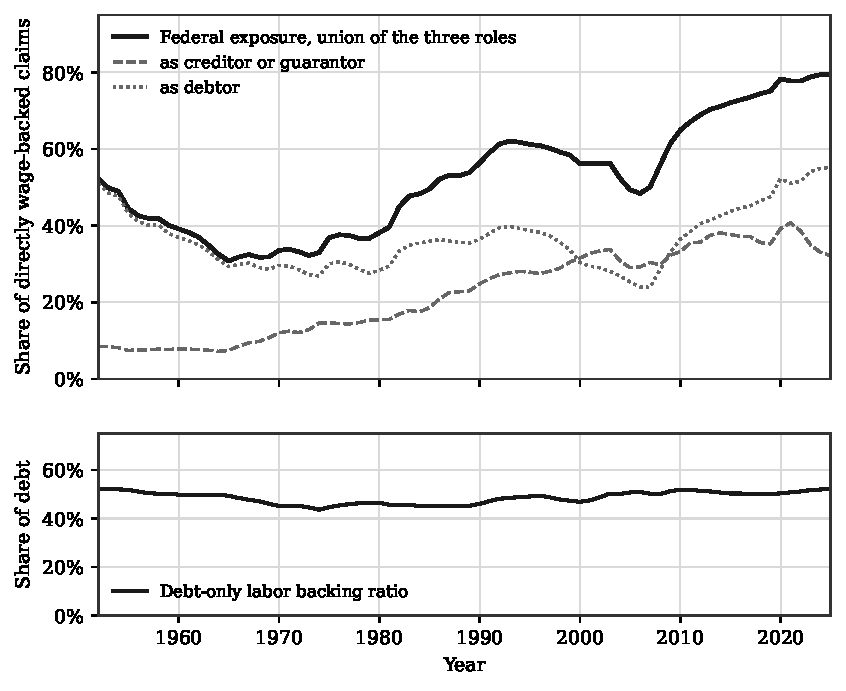
\includegraphics[width=0.86\textwidth]{fig1_series.pdf}
\caption{Federal exposure to directly wage-backed claims, 1947 to 2025, and the debt-only labor backing ratio, 1952 to 2025. The two panels open in different years because the debt-only ratio needs market-valued equity, which the accounts carry only from 1952. Upper panel: the exposure share as the union of the three roles, with its creditor or guarantor and debtor parts, which overlap where the federal sector holds its own debt and so do not sum to the union. Lower panel: the share of US debt attributed to labor income on the direct route. Both panels are on the coverage construction of the household coefficients, because income by source is not available for the historical years. Measured, from the Federal Reserve financial accounts.}
\label{fig:series}
\end{figure}


\subsection{The other side, reported as bounds}
\label{sec:aiside}

The same decomposition applied to claims on AI capital gives the comparison the paper is for, and
it is reported as bounds rather than as a point, because the two sides are not equally observable.
The wage side is a measured stock. The AI side is assembled in tiers: a measured lower bound of
\result{OnBalanceSheetAIDebtBn} billion dollars of on-balance-sheet debt from nine registrants'
filings, about \result{AIBankCommitmentsBn} billion dollars of bank commitments to AI-adjacent
industries, a scenario tier for AI-attributable equity swept at \result{AIEquityScale} percent of
nonfinancial corporate equity, and an unmeasured tier of off-balance-sheet vehicles,
hardware-backed lending and securitizations, which \citet{BIS2026} describes as dominant and which
contributes nothing to our total.

The federal share of that side is \result{AIFederalShareLow} to \result{AIFederalShareHigh}
percent across a threefold variation in the assumed scale, about
\result{AIFederalShareRounded} percent at the central value. The level is a lower bound, since
the unmeasured tier would enlarge it. The share is an upper bound only under a stated assumption:
that the federal government's share of the omitted assets does not exceed its share of the
observed ones. That is plausible because the omitted financing is private credit, securitizations
and vendor finance, which the federal sector holds and guarantees far less of than it does the
claims it already holds here, but it is an assumption and not a measurement. If instead the
federal share of the omitted assets equalled its share of the observed ones, the federal share of
the whole AI side would stay at about \result{AIFederalShareRounded} percent rather than falling
below it.
Figure~\ref{fig:holders} puts the two sides beside each other.

What the comparison does and does not say is worth stating carefully, because the two numbers are
different economic objects. The wage-side share counts three roles on one pool of claims: what the
federal government holds, what it guarantees and what it owes out of wage-financed receipts. The
AI-side share is an ownership share of a different pool. Their difference, about
\result{HolderGap} percentage points, is therefore a statement about where exposure sits, not a
portfolio imbalance and not a measure of how well the state is hedged. Whether the state's
position is adequate has to be asked in common dollars over a common period, a separate question,
and one a companion paper takes up on these same accounts \companion.

\begin{figure}[htbp]
\centering
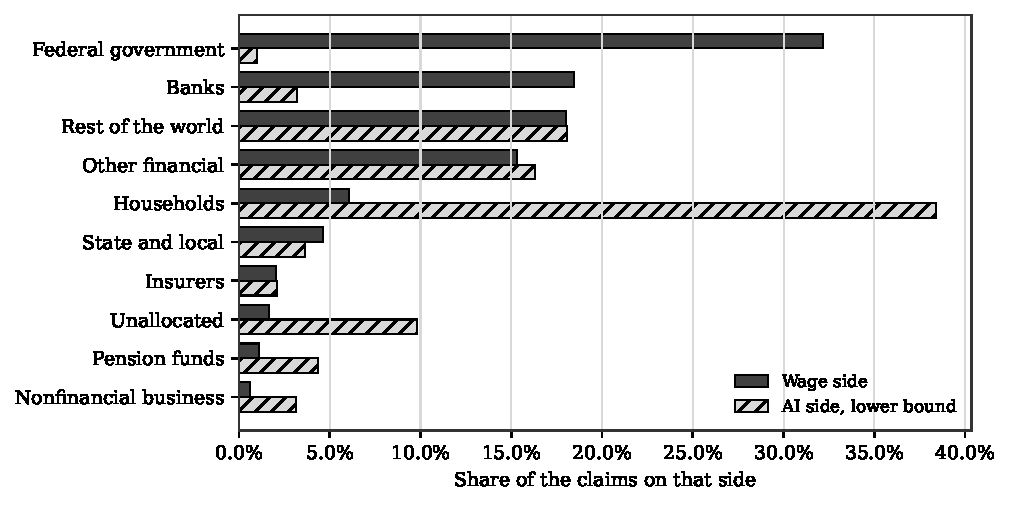
\includegraphics[width=0.84\textwidth]{fig2_holders.pdf}
\caption{Holders of the two sides. The wage side is the measured stock of directly wage-backed
claims; the AI side is a lower bound built from on-balance-sheet filings with a scenario scale for
AI-attributable equity. Because the total is incomplete, a given holder's share is an upper bound
only if that holder's share of the omitted claims is no larger than its share of the measured
ones; for a holder over-represented in the omitted tier the printed share is a lower bound. We
argue that condition for the federal share in Section~\ref{sec:aiside} and do not assert it for
the others. The federal
government is the largest holder on one side and close to absent on the other.}
\label{fig:holders}
\end{figure}


\section{Households, by position in the wage distribution}
\label{sec:households}

The accounts carry one more cut. Because the household part of the wage-backed stock can be split
by wage quintile, and because the same survey gives the liquid assets of the same households, the
two can be set side by side. They answer different questions and they disagree, which is the
result of this section.

\subsection{Claims are spread more evenly than the income that services them}

The gradient is the finding: wage-backed claims per dollar of wages fall as pay rises, from
\result{QTwoPerDollar} in the second quintile to \result{QTopPerDollar} at the top, while the top
quintile earns \result{QTopWageShare} percent of the wage bill and carries
\result{QTopClaimShare} percent of the household claims. Claims are spread far more evenly than
the income that services them. Table~\ref{tab:quintile} gives the detail, and
Appendix~\ref{app:detail} the construction, including the one magnitude the accounts can produce
but that we do not report.

That is the sense in which a proportional fall in pay is regressive before any policy response is
chosen. It is an arithmetic property of the claim structure, not a claim about how anyone
behaves. A household in the second quintile supplies about nine percent of the wage bill and
carries about thirteen percent of the household claims against it; a household in the top
quintile supplies half the wage bill and carries a third of the claims. Nothing has to happen for
that asymmetry to exist. It is there now.

\subsection{Where the buffers are thinnest, and it is not the bottom}

Liquid runway by wage quintile gives the second household result, and buffers are not monotonic
in pay: the thinnest are in the \emph{second} quintile, a median of \result{QTwoRunway} months
against \result{QOneRunway} in the bottom quintile, with \result{QTwoUnderOne} percent under one
month against \result{QOneUnderOne} percent. From there upward the gradient is monotonic,
reaching \result{QFiveRunway} months at the top. Bottom-quintile households hold little debt and
few of the commitments a runway is measured against, while second-quintile households carry the
commitments of those above them without the income to service them, so relief targeted at the
bottom of the distribution misses the households with the least room.

\begin{table}[htbp]
\centering
\caption{Liquid runway of working households by wage quintile: months of income covered by liquid
assets, and the share with less than one month. Measured.}
\label{tab:buffers}
\input{tables/tab_buffers.tex}
\end{table}

\subsection{What the two cuts say together}

The claims gradient and the buffer gradient are measured on the same households from the same
survey, and they do not line up. Claims per wage dollar peak one quintile above the bottom.
Liquid runway bottoms out in the same place. The households carrying the most debt per dollar of
income earned are also the households with the least room to absorb a gap in that income, and
neither fact is visible in a statistic that ranks households by income alone or by wealth alone.

We state this as a measured coincidence rather than as a mechanism. The accounts cannot say why
the second quintile occupies that position, and a plausible reading, that these are households
with enough income to qualify for credit and not enough to build a buffer against it, is a
hypothesis this paper does not test. What the accounts establish is the location. Anything
targeted at the bottom of the wage distribution, whether credit policy, relief or disclosure,
is aimed one quintile away from the thinnest margin in the household sector.


\section{Implications for Individuals, Organizations, and Society}
\label{sec:implications}

A measurement is only worth the decisions it improves. This section sets out what follows from
the accounts for the people the exposure reaches, for the organizations that have to govern it,
and for the wider public interest. We separate what the evidence supports from what it does not,
because recommendations are the easiest part of a paper of this kind to overreach.

\paragraph{For the people the exposure reaches.} The household that services a mortgage, a car
loan and a student loan out of one wage is not an edge case in this system; it is the system's
modal unit. Our measurements place it there. One practical consequence is that liquid assets
relative to income are not monotonic in pay: measured that way they are lowest one quintile above
the bottom, among households carrying the commitments of those above them without the income to
service them. We stop short of calling those households the most vulnerable, because that
depends on expenditure and commitments the accounts do not carry, but a relief design that
assumes liquidity rises with pay is assuming a pattern the data do not show. Relief designed
around occupation faces a separate problem: the accounts show the exposure is spread almost
evenly across borrowers rather than concentrated in identifiable jobs.

There is a second consequence, and it runs the other way. Because the claims are spread more
evenly than the wages, the exposure is not concentrated in a group that could be identified and
advised. We are careful about what follows. The accounts measure a stock and its attribution;
they do not survey the instruments available to a household, so they cannot establish that no
such instrument exists. What they do establish is narrower: the exposure is common rather than
sorted, so any remedy that works by identifying the exposed will have little to sort on. Whether
public instruments or disclosure are the right answer is a question about costs and
counterfactuals that these accounts do not price.

\paragraph{For managers and organizations.} The governance question these accounts pose is
narrow and answerable: can an institution state, in a form a board can read, how much of its
income and collateral depends on wages continuing to be paid? Most cannot, because no standing
statistic reports it. That is a measurement gap an institution can close for itself from its own
book using the coefficients in Table~\ref{tab:bridge}, and the exercise is cheap.

What the evidence does \emph{not} support is tightening household underwriting in response. Three
measured grounds stand against it: the debt service result is partly mechanical, since
underwriting already caps debt service to income; the exposure is spread almost evenly across
borrowers, so screening on it buys a lender little; and the one pre-registered institutional
test we ran was a null, which Section~\ref{sec:limitations} reports in full. That last point
is a null on one outcome in one window, not a demonstration that the accounts can never carry
institution-level predictive content, and we do not read it as the stronger claim. Wage
dependence is a concentration to be governed and disclosed, not a credit category to be
underwritten.

\paragraph{Strategic implications.} The holder map makes an ownership question explicit that is
usually left implicit. If every holder class carries wage-attributed claims in some proportion,
then hedging inside the system requires a counterparty whose own exposure is lower, and the map
says which classes those would be rather than that none exist. We do not claim the exposure
cannot be diversified away, and we do not rank instruments: the accounts carry no prices, no
contract terms and no costs, so a statement that one instrument has the best ratio of value to
cost is not available from them. What the map supports is weaker and still useful: an
institution can read its own wage-attributed share off a published construction, which makes the
number auditable rather than discretionary.

The second strategic point concerns timing. The federal share of the wage-backed stock has
more than doubled from its trough, \result{SovUnionTrough} percent in \result{SovUnionTroughYear} against
\result{SovereignUnion} percent in 2025, a factor of \result{SovUnionRiseFromTrough}. Across the whole series it
has not doubled: it was \result{SovUnion1947} percent in 1947, so the series is a U and the rise is
from the middle of it rather than from the start. The whole net increase since 2008 sits in the
debtor position rather than in new guarantees. A position acquired that way is acquired without a
decision having been taken about it. Making it visible is the precondition for deciding whether
to keep it.

\paragraph{For society and equity.} The claims that wages pay are spread far more evenly than the
wages themselves. The implication is a balance-sheet one and we keep it there: a proportional
fall in pay lands against claim stocks that are larger relative to wages further down the
distribution, so the ratio of claims to wages rises as pay falls. That is not the same as showing
the fall is regressive in welfare, in default or even in debt service, each of which depends on
payment schedules, maturity, transfers, other assets and expenditure, none of which these
accounts carry. What the structure of the claim stock settles is the gradient of the stock. The
incidence of a shock on wellbeing or on arrears is a further question and we do not answer it
here.

Two refusals belong here as well, because a statistic that locates wage risk could be used
against the people it describes. These accounts are built at the level of claim classes and
holders, not individuals, and nothing in them supports pricing a person's credit by what they do
for a living. Occupation is not a prohibited basis under the Equal Credit Opportunity Act, whose
list of prohibited bases does not include it, but because occupation correlates with protected
classes, occupation-based underwriting in housing credit exposes a lender to a
discriminatory-effects claim under the Fair Housing Act, on which the lender must carry a legally
sufficient justification. Combined with the finding that the exposure is spread almost evenly
across borrowers, the risk-adjusted case for it is weak and the case for portfolio-level
disclosure is strong. A statistic that locates wage risk should size public instruments. It
should not price individuals out of credit for what they do for a living.


\section{Limitations}
\label{sec:limitations}

Every limitation below is numbered so that the avenues in Section~\ref{sec:future} pair with it
one to one. We state them plainly. An accounting framework that overstates its reach is itself a
hazard, because the number it produces looks authoritative in exactly the settings where it is
weakest.

\paragraph{L1. The accounts are not a risk measure, and we tested that.} This is the limitation
that most constrains what the framework is for, so it goes first rather than last.

Under a pre-registered design fixed before any outcome was opened, we tested whether labor
backing measured before the 2014 to 2016 oil price collapse predicts subsequent household-loan
charge-offs across about \result{NBanks} US banks beyond conventional measures. It does not. The
debtor-specific component that is distinctive to the accounts had no predictive content, neither
it nor the public rival improved out-of-sample prediction in held-out states, and the design's
own pre-shock placebo failed under the standard errors we had named as governing, so that episode
supports no causal reading in either direction.

A second pre-registered test, on a much larger sample, reached the same place by a different
route. Across \result{PredPanelRows} bank-years covering \result{PredPanelBanks} banks from 2001
to 2024, forward-chaining out-of-sample over \result{PredPanelYears} test years, adding the
measure to a conventional bank-risk model raised the out-of-sample $R^2$ by
\result{PredRawDrTwo}. That apparent gain does not survive inspection: the baseline's own
out-of-sample $R^2$ is negative in ten of the thirteen years, so a positive increment can be
earned by correcting the level rather than by ordering the banks. Re-centring both predictions on
the test-year mean removes that level difference and moves the increment to
\result{PredRecentredDrTwo}; it does not isolate ranking, because a centred squared error still
responds to the scale and dispersion of the predictions. The direct test of ranking is the
cleaner one: the
out-of-sample rank correlation between prediction and realized charge-off rate falls from
\result{PredRhoControls} with conventional controls alone to \result{PredRhoWith} once the
measure is added, and it improves in \result{PredYearsImproved} of \result{PredPanelYears} test
years. The debtor-specific variant improves in \result{PredGapYearsImproved} of
\result{PredPanelYears}.

The reason is visible in the construct's own algebra rather than only in the outcomes. Because
the class coefficients are close to binary, about 0.80 on every household class and zero on every
business class, the bank-level measure is largely a restatement of how much household lending an
institution does. Regressing it on the seven conventional loan-share controls alone gives an
$R^2$ of \result{PredCollinearityRSq}. That makes the result unsurprising, and it is worth being
careful about what it does and does not imply. It does not imply that the residual variation is
uninformative: a measure half explained by a set of controls can in principle carry predictive
content in the other half. What it establishes is that the measure is substantially a restatement
of information the baseline already has, which is a reason to expect a small increment, not a
proof that none exists. The claim we make is the empirical one, that in these two tests the
increment was absent and the ranking got worse, not the general one that it must be.

We therefore present labor backing accounts as aggregate accounting of where wage dependence
sits, and not as an institution-level risk measure. The pre-registrations, amendments, deviations
logs and results for both tests are archived with the replication package.

\paragraph{L2. Off-balance-sheet and hardware-backed AI financing is unmeasured.} The side of the
accounts measuring claims on AI capital is built from nine registrants' on-balance-sheet facts.
Off-balance-sheet vehicles, which \citet{BIS2026} identifies as dominant in data center
financing, contribute nothing to it, and neither does hardware-backed lending or securitization.
Every level on that side is a lower bound and every federal share of it an upper bound, which is
why Section~\ref{sec:accounts} reports it as bounds rather than as a point.

\paragraph{L3. Capital gains inside federal receipts are not separated.} Realized gains sit
inside the base we split by the wage share of adjusted gross income, so the labor-linked share
overstates in years with large realizations and understates in years without. The band is carried
throughout and the federal exposure share moves by under one percent across it.

\paragraph{L4. The holder split leaves an unidentified remainder.} Three of the four shares in
the mortgage holder split are read from a publisher and the fourth is an arithmetic remainder,
treated as private in full. That is conservative for our claim, since any federal fraction inside
it would raise the federal share, but we have not identified what is in it, and the AI side has a
remainder of the same kind.

\paragraph{L5. The historical series rests on the coverage construction.} Income by source is not
available for the historical years, so the series from 1952 and the sensitivities computed
against it use the coverage construction of the household coefficients rather than the adopted
wage basis. The two agree within \result{CoefficientMaxMovePP} percentage points on every
coefficient at the one date where both can be computed, but that agreement is assumed to hold
backwards and cannot be checked.

\paragraph{L6. One distributional magnitude is withdrawn.} Wage-backed claims per wage dollar in
the bottom quintile is not reported. An independent rebuild landed a factor of two and a half to
three and a half away, and we cannot show their reading is wrong, because our own specification
defined neither the universe nor the normalization of that cell. The gradient was reproduced and
stands; this one magnitude does not. Table~\ref{tab:removed} lists it with four others.

\paragraph{L7. The novelty of the accounts is ``none located'', not ``none exists''.} A search
with a stated protocol has now been run. It fixed in advance what would count as a precedent,
namely a construction that takes a national claim stock, classifies each claim by the income that
services it, crosses that with the holder structure and reports an aggregate share, and it fixed
in advance that locating one would retire the novelty claim. None was located. The nearest
neighbours are named in Section~\ref{sec:related} with the condition each fails.

The bounds of that search are the limitation. Six queries against a general web index is a
documented search, not an exhaustive one: it does not systematically cover paywalled journal
archives, non-English literature, statistical agency working papers that are not web indexed, or
unpublished central bank work. Any of those could hold a precedent. The related-work audit did
locate prior work on the fiscal mechanism and that priority claim was retired; the same could
still happen here. The protocol, the queries and the neighbours are archived with the replication
package.

\paragraph{L8. The accounts are built for one country.} Every result here is for the United
States. A federal share near four fifths may be a property of this state, or of any state running
large mortgage guarantee programs and funding itself from payroll taxes, and one country cannot
tell the two apart. We attempted a euro-area counterpart and did not reach the standard of the US
series, because the published counterpart detail there does not support the issuer-side leg of
the holder map; that attempt is recorded rather than reported.

\paragraph{What a rebuild does not establish.} The independent computational rebuilds described
in Section~\ref{sec:rebuild} and Appendix~\ref{app:rebuild} establish that the stated inputs and
the stated construction produce the stated numbers. They do not establish that the constructions
are the right ones, or that the economic assumptions behind them hold. The blind was procedural
rather than enforced, which is why this paper says these quantities were independently rebuilt
under a reported blind protocol and never that they were independently verified.


\section{Avenues for further research}
\label{sec:future}

Each avenue below addresses the limitation carrying the same number in
Section~\ref{sec:limitations}.

\begin{description}[leftmargin=2.4em,style=nextline]

  \item[FR1] Researchers should test whether the accounts carry information at a level of
  aggregation where loan composition does not already dominate, such as the county or the
  program, rather than at the level of an individual intermediary where we have shown they do
  not. The two nulls we report both bite at bank level, and the reason they bite there, that the
  measure is largely a restatement of loan mix across institutions, does not obviously apply to a
  geography whose employers differ while its loan mix does not.

  \item[FR2] Researchers should build the off-balance-sheet side of the AI claim stock from
  securitization prospectuses, vehicle-level filings and supervisory data on lending secured
  against computing hardware, so that side can be measured rather than bounded, and the holder
  comparison can be made on two measured stocks rather than one measured and one bounded.

  \item[FR3] Researchers should separate realized capital gains from wage income inside the
  individual income tax base and recompute the Treasury coefficient on the separated series,
  which would replace the band we carry with a point and tighten every fiscal magnitude that
  depends on it.

  \item[FR4] Researchers should identify the mortgage holder remainder from loan-level sources
  rather than leaving it as an arithmetic residual treated as private in full, which would
  establish whether the federal share we report is conservative by a little or by a lot.

  \item[FR5] Researchers should reconstruct income by source for the historical years from tax
  and survey microdata, which would let the whole series be placed on the adopted wage basis and
  remove the assumption that the two constructions stay close going backwards.

  \item[FR6] Researchers should define the universe and the normalization for the bottom-quintile
  cell explicitly and recompute it, so the one withdrawn distributional magnitude can be restored
  or ruled out rather than left absent.

  \item[FR7] Researchers should extend the novelty search into the archives this one did not
  reach. The protocol is published and the search has been run against a general web index with
  a stated kill criterion, which is what converts ``none located'' from an admission into a
  result. What it does not reach is paywalled journal archives searched systematically rather
  than by query, non-English literature, statistical agency working papers outside the web index
  and unpublished central bank work. A librarian-assisted search across those four would settle
  the question in a way a web search cannot.

  \item[FR8] Researchers should construct labor backing accounts for a second country on the same
  basis. The United States is one observation, and whether a federal share near four fifths is a
  property of this state or of states with large mortgage guarantee programs generally cannot
  be settled from one country. Our own attempt at a euro-area counterpart did not reach the
  standard of the US series, because the published counterpart detail does not support the
  issuer-side leg, so this needs national sources country by country rather than a single
  harmonized release.

  \item[FR9] Researchers should put the whole accounts on a single vintage of the federal
  receipts aggregates. The Treasury coefficient is currently computed on the 2025 national
  accounts while the capital-gains band and the quoted receipts base come from a different
  vintage, so the two differ by about two percentage points for reasons that have nothing to do
  with the construction. One vintage throughout would remove that.

\end{description}


\section{Conclusion}
\label{sec:conclusion}

The financial accounts of the United States have described the claim structure as a matrix of
counterparties for seventy years. They do not record which income services each claim, and that
omission hides a position nobody chose to take.

Decomposed by servicing income, about \result{DebtOnlyDirect} percent of all US debt, public and
private, is paid directly out of wages, and \result{DebtOnlyIndirect} percent once indirect
servicing is counted. Crossed with the holder structure, the same decomposition shows the federal
government standing behind about \result{SovereignUnion} percent of the directly wage-backed
claims as holder, guarantor or debtor, against about \result{AIFederalShareRounded} percent of
the separately measured claims on AI capital. Counting only what the public sector holds
understates that position by more than a factor of two, which is why the headline carries its
convention wherever it appears.

The long series puts the present level in its place. The federal share traces a U, from
\result{SovUnion1952} percent in 1952 through \result{SovUnion1970} percent in
1970 to \result{SovUnion2025} percent in 2025, so today is a return rather than a
record, and a large part of the recent rise is growth in federal debt itself rather than new
exposure to households. The ratio underneath it is close to flat across seventy-three years. The
share of the national debt stock that wages service is not a recent development.

Across the wage distribution, claims are spread far more evenly than the income that services
them, and the thinnest liquid buffers sit one quintile above the bottom rather than at it. A
proportional fall in pay is therefore regressive before any policy response is chosen, and relief
designed around the bottom of the distribution is aimed one quintile away from the least room.

What the accounts do not do is predict. Two pre-registered tests, the second on
\result{PredPanelRows} bank-years, found that adding the measure to a conventional bank-risk
model makes out-of-sample ranking worse rather than better. We report both because they bound the
contribution: this is accounting that says where wage dependence sits, not a measure that says
which institution will take a loss. Every number here is generated from an artifact in a
replication package, each carrying its status, so a reader who rejects a convention can change it
and see exactly what moves.


\section*{Declarations}

\paragraph{Data availability.} The replication package, containing the measured artifacts behind
every reported value and the code that generates them, will be public at a named repository on
publication. During review it is private and is available to referees and editors on request
through the journal. The validation pilot reported in Section~\ref{sec:limitations} is archived
alongside it as four documents, the pre-registration with its amendments, the deviations log, the
results and the close-out note; its code and data are not part of the package.

\ifanon
\else
\paragraph{Disclosure statement.} The authors report no conflict of interest.
\paragraph{Funding.} This research received no external funding.
\fi

\paragraph{Use of generative AI.} The authors set the research questions, directed the work, and reviewed and approved every
methodological decision. Many of those decisions, including definitions, conventions and checks,
were proposed by generative AI tools, which also wrote the analysis code, carried out the
independent computational rebuilds from published specifications, and drafted the text. The
authors take responsibility for the content of the paper. No reported value originates in a
model's assertion: every number in the text and in the tables is generated from a measured
artifact in the replication package.


\appendix

\section{The independent computational rebuilds}
\label{app:rebuild}

Three rebuild rounds have been run against the measurements in this paper. Each was carried out by
a separate run with no access to the project's code, working from raw data and a published
specification, and scored against expected values fixed before the round began.

Round one established the protocol and produced no comparable values in several modules, because
the specification it worked from left definitions unstated. Round two scored
\result{RepTwoScored} quantities, \result{RepTwoSealed} of them against fixed expected values:
\result{RepTwoFivePct} came within five percent and \result{RepTwoTolerance} inside the stated
tolerance, while \result{RepTwoMismatch} did not match. The mismatches had six root causes, of
which the largest were an undefined universe for one household object, a class omitted because the
specification described the exclusion rule in prose without enumerating the classes, and a
Treasury level the rebuild could not know was the sum of two published series. Three of the five
quantities withdrawn from this paper were withdrawn as a direct result. Round three covered the
two constructions the earlier rounds had not reached, the debt-only ratio and the assembled
capital tax rate, and matched all \result{RepThreeSealed} quantities,
\result{RepThreeRounding} within rounding and the remainder inside tolerance. Its two
non-rounding matches were traced exactly: one to a central value taken at a range midpoint rather
than at the sourced point, which the paper now reports at the sourced point, and one to the
maximum of a finite sample over a seven-dimensional box, which is an extreme order statistic with
no stable value and is now reported as the analytic corner instead.

The blind was procedural rather than enforced. The rebuild ran on the same machine, with the file
of expected values reachable at a path the specification names; it was not attached to the request
and was reported unopened until the rebuild was final. The supporting evidence is internal and
circumstantial: most insufficiencies were written before the file was opened, several of the
mismatch causes were among them, and the rebuild declined to use coefficients the specification
had leaked. On that basis the paper claims that these quantities were independently rebuilt under
a reported blind protocol, and never that they were independently verified.


\section{Further detail on the accounts}
\label{app:detail}

The material below was moved out of the body for length. Nothing in it is altered.

\subsection{The two conventions in the accounts}

\emph{Supporting Section~\ref{sec:accounts}, on the two conventions the accounts rest on.}

\paragraph{Government debt enters by its receipts, not by its obligor.} Treasury debt is not
wage-backed because a household owes it, but to the extent that wage taxes service it, so it takes
the labor-linked share of federal receipts, social insurance contributions in full plus the wage
share of the individual income tax, measured at \result{TBResult} on the adopted vintage; state and local
debt is treated the same way on its own receipts mix. Without this convention a government funded
entirely from payroll taxes and one funded entirely from capital taxes would score identically.

\paragraph{The one-step rule is a convention, and it is the largest judgment in the paper.} We
trace servicing one step and stop, so a claim serviced out of business revenue takes zero direct
backing even though some of that revenue began as wages. Multifamily mortgages are the one
property class that does not take the zero, because the rent that services them is paid out of
wages with no firm in between. The rule is the first-round boundary applied to the liability side.
Tracing further is what the indirect variant does, and we report both: on the whole claim stock,
moving business classes to their measured indirect share raises the ratio by
\result{OneStepMoveAllClaimsPct} percent, more than every other judgment call in the accounts
together.

\subsection{The series, 1947 to 2025}

\emph{Supporting Section~\ref{sec:accounts}, on the path of the accounts since 1947.}

Figure~\ref{fig:series} runs the accounts back to 1947, and two things in it move differently.
The two panels open in different years: the holder structure can be built from 1947, while the
debt-only ratio needs market-valued equity and starts in 1952.

The ratio itself is close to flat across the seventy-three years it covers, between
\result{DebtOnlySeriesLow} and \result{DebtOnlySeriesHigh} percent on the debt-only measure with
no trend. The share of the national debt stock that wages service is not a recent development.

The federal share of it traces a U: \result{SovUnion1947} percent in 1947,
\result{SovUnion1952} percent in 1952, \result{SovUnion1970} percent in 1970,
\result{SovUnion2025} percent in 2025. The post-war opening is almost entirely wartime Treasury
debt, the debtor position alone standing at \result{SovObligor1947} percent in 1947 against a
creditor leg of \result{SovHeld1947} percent, and it is still
\result{SovObligor1952} percent in 1952. It falls to 1970 as that debt shrinks against a growing claim
stock, then climbs in two datable steps: the agency book grows between 1970 and 1990, taking the
held-or-guaranteed position from \result{SovHeld1970} to \result{SovHeld1990} percent, and federal
debt grows between 2008 and 2020, taking the debtor position from \result{SovObligor2008} to
\result{SovObligor2020} percent.

Said plainly, because it qualifies the headline: a large part of the recent rise is growth in
federal debt itself rather than new exposure to households. The held-or-guaranteed position peaked
at \result{SovHeld2020} percent in 2020 and has since fallen to \result{SovHeld2025} percent,
while the whole net increase since 2008 sits in the debtor position.

\subsection{Households, by position in the wage distribution}

\emph{Supporting Section~\ref{sec:accounts}, on the household part of the wage-backed stock.}

Splitting the household part of the stock by wage quintile gives the gradient: wage-backed claims
per dollar of wages fall as pay rises, from \result{QTwoPerDollar} in the second quintile to
\result{QTopPerDollar} at the top, while the top quintile earns \result{QTopWageShare} percent of
the wage bill and carries \result{QTopClaimShare} percent of the household claims. Claims are
spread far more evenly than the income attributed to servicing them, so the ratio of claims to
wages rises as pay falls. That is a statement about the stock and not about welfare incidence. Appendix Table~\ref{tab:quintile} gives
the detail.

The magnitude for the bottom quintile is reported with its dispute flagged, for the
reason given at L6 in Section~\ref{sec:limitations}: an independent rebuild lands
two and a half to three and a half times lower, and because that range straddles the second
quintile the bottom quintile's rank is not established. The decline from the second quintile
downward was reproduced and stands.


\section{Additional tables}

\begin{table}[htbp]
\centering
\caption{Labor backing and federal exposure, selected years, 1947 to 2025. The debt-only ratio
reads n/a for 1947 because it needs market-valued equity, which the accounts carry only from
1952. Computed on the
coverage construction of the household coefficients, because income by source is not available for
the historical years; the 2025 row therefore differs slightly from the headline figures, which are
on the adopted wage basis. The creditor and debtor columns overlap where the federal sector holds
its own debt, so they do not sum to the union. Measured, rebuilt.}
\label{tab:series}
\input{tables/tab_series.tex}
\end{table}

\begin{table}[htbp]
\centering
\caption{Federal exposure under alternative structural choices, computed on the coverage
construction for the reason given in Section~\ref{sec:accounts}; the moves, not the levels, are
what the table reports. Measured, rebuilt.}
\label{tab:structural}
\input{tables/tab_structural.tex}
\end{table}

\begin{table}[htbp]
\centering
\caption{Wage-backed household claims by wage quintile, on the adopted wage basis. Claims per
wage dollar is the share of household wage-attributed claims divided by the share of the wage
bill. The fourth column uses the wage-bill share from the American Community Survey, as
published; the fifth recomputes it from the same survey file as the balances, as workers times
mean wage, so that numerator and denominator share one universe. The two differ by at most
\result{QuintDenomDivergence} percent anywhere and by \result{QOneAgreement} percent at the
bottom. $\dagger$ the bottom-quintile magnitude remains contested: an independent rebuild lands
at 1.21 to 1.64 and we cannot reproduce its construction, so that quintile's rank is not
established. See L6 in Section~\ref{sec:limitations}. Measured.}
\label{tab:quintile}
\input{tables/tab_quintile.tex}
\end{table}

\begin{table}[htbp]
\centering
\caption{Quantities removed from or contested in this work, with the reason for each.}
\label{tab:removed}
\input{tables/tab_removed.tex}
\end{table}

\bibliographystyle{apalike}
\bibliography{references}

\end{document}
